%\documentclass[conference, oribibl]{IEEEtran}
\documentclass[runningheads,a4paper,oribibl]{llncs}
\usepackage{llncsdoc}

% *** MISC UTILITY PACKAGES ***
%
\usepackage{amssymb}
\setcounter{tocdepth}{3}

\usepackage{graphicx}
\graphicspath{ {Figs/} }

\usepackage{amsmath}
\usepackage{multirow}
\usepackage{slashbox}
\usepackage{amsfonts}

\usepackage{algorithm2e}
\usepackage{epstopdf}
\usepackage{array}
\usepackage{enumerate}

\usepackage{epstopdf}

\usepackage{url}
%\urldef{\mailsa}\path|{khanhtv, mizuhito}@jaist.ac.jp|    

%ieee requirements
%\usepackage[utf8]{inputenc}
%\usepackage[T1]{fontenc}
%\usepackage{microtype} 
%\usepackage{balance}

%user definitions
\newcommand{\Nat}{{\mathbb N}}
\newcommand{\Real}{{\mathbb R}}
\newcommand{\Rat}{{\mathbb Q}}
\newcommand{\suppress}[1]{} % Comment out text.
\newcommand{\mizuhito}[1]{\{{\bf Mizuhito:~\sf #1}\}} % Highlight text.
\newcommand{\khanh}[1]{\{{\bf Khanh:~\sf #1}\}} % Highlight text.

\newcommand{\smallHead}[1]{%
    \par\vspace{.35cm}\noindent\textbf{#1}%
    \par\noindent\ignorespaces%
}

\newcommand\TTTT{%
 \textsf{T\kern-0.2em\raisebox{-0.3em}T\kern-0.2emT\kern-0.2em\raisebox{-0.3em}2}%
}

% correct bad hyphenation here
\hyphenation{op-tical net-works semi-conduc-tor}


\begin{document}
%
% paper title
% can use linebreaks \\ within to get better formatting as desired
% Do not put math or special symbols in the title.
\title{{\bf raSAT}: SMT for Polynomial Inequality}

\author{To Van Khanh\inst{1} and Mizuhito Ogawa\inst{2}} 
\institute{University of Engineering and Technology, Vietnam National 
University, Hanoi \\
\email{khanhtv@vnu.edu.vn}
\and 
Japan Advanced Institute of Science and Technology\\
\email{mizuhito@jaist.ac.jp}
}

% make the title area
\maketitle

% As a general rule, do not put math, special symbols or citations
% in the abstract
\begin{abstract}
This paper presents an iterative approximation refinement, called {\bf raSAT} loop, 
which solves a polynomial inequality on real numbers.
The approximation scheme consists of interval arithmetic 
(over-approximation, aiming to decide UNSAT) and 
testing (under-approximation, aiming to decide SAT). 
If both of them fail to decide, input intervals are refined by decomposition. 

The {\bf raSAT} loop is implemented as an SMT {\bf raSAT} with miniSAT 2.2 as 
a backend SAT solver. 
Experiments are performed on QF\_NRA benchmarks from SMT-LIB and 
simple benchmarks intending to estimate effects of input measures 
(i.e., degrees, number of variables, and number of polynomials). 
They show that {\bf raSAT} is comparable to Z3 4.3, and sometimes outperforms, 
especially with high degree of polynomials.
%For instance, 
%polynomial inequality with a long monomial (e.g., $60$), degree $6$, and 
%many variables (e.g., $14$) in Zankl family are such examples. 

\suppress{
Experiments are performed on simple benchmarks to estimate effects of input measures, 
(the degree of polynomials, the number of variables, 
and the number of atomic polynomial inequalities), and benchmarks of QF\_NRA category 
in SMT-LIB. Results show that {\bf raSAT} is comparable and sometimes outperform 
Z3 4.3, which is believed to be one of the strongest SMT solvers on QF\_NRA category.  
}
\end{abstract}

% no keywords
%\keywords{interval arithmetic, affine arithmetic, SMT, polynomial constraints, 
%testing, abstract DPLL.}


% For peer review papers, you can put extra information on the cover
% page as needed:
% \ifCLASSOPTIONpeerreview
% \begin{center} \bfseries EDICS Category: 3-BBND \end{center}
% \fi
%
% For peerreview papers, this IEEEtran command inserts a page break and
% creates the second title. It will be ignored for other modes.
% \IEEEpeerreviewmaketitle

\section{Introduction}
{\em Polynomial constraint solving} is to find an instance 
that satisfies given polynomial inequality/equality. 
For instance, $\exists x y. -y^2 + (x^2 - 1) y - 1 > 0 \wedge -x^2 - y^2 + 4 > 0$ is 
such an example. This is an easy formula, but proving its satisfiability and showing a satisfiable instance (e.g., $x = 1.8$, $y=0.9$) are not so easy.  
%its satisfiability and a satisfiable instance 
%(e.g., $x = 1.8$, $y=0.9$) are not so easy.  		

Many applications are reduced to solving polynomial constraints, such as 
\begin{itemize}
\item {\bf Locating roundoff and overflow errors}, 
which is our motivation~\cite{ngocsefm,ngocase}. 
DSP decorders in practice are defined by reference algorithms in C using floating point arithmetic. 
In embedded systems, often it is replaced with fixed point arithmetic, 
which may cause visible noises. 
%and locating such roundoff error source is not easy. 
%For instance, consider DSP decoder like mpeg4. Usually, the decoder definition is given by a reference 
%algorithm in C, which uses floating point number. 
%In an embedded system, it is tempting to replace floating 
%point into fixed point numbers. However, naive replacement would cause 

\item {\bf Automatic termination proving}, 
e.g., \TTTT~\footnote{\url{http://cl-informatik.uibk.ac.at/software/ttt2/}}, 
Aprove~\footnote{\url{http://aprove.informatik.rwth-aachen.de}}. 
is reduced to finding a suitable termination ordering~\cite{lucas}. 
%as a solution of polynomial constraints. 

\item {\bf Loop invariant generation}.
Farkas's lemma is a popular approach in linear loop invariant generation~\cite{Colon03}, 
and is reduced to degree $2$ polynomials. 
%matrix multiplications. 
%degree $2$ polynomial constraints. 
%Farkas's lemma uses products of matrices, and it requires solving polynomial constraints of degree 2.
Non-linear loop invariant~\cite{Sankaranarayanan} requires more complex polynomials.

\item {\bf Hybrid system}. SMT for QF\_NRA are often used as backend engines~\cite{hybrid}. 

\item {\bf Mechanical contrnol design}. 
PID control is simple but widely used, and designing parameters is 
reduced to polynomial constraints~\cite{control}. 
%Fujitsu used polynomial constraints solving to design PID control of HDD head movement
\end{itemize}	

%Our approach is based on the first category. 
We focus on polynomial inequality, which simplifies problems a lot still 
keeping applications. 
This view is shared with $\delta$-completeness~\cite{dRealIJCAR12,dRealLICS12}. 
\begin{itemize}
\item %In constructive analysis, 
Inequality $a < b$ on real numbers is computable 
whereas equality $a = b$ is not. ($a=b$ can be decided for algebraic numbers by 
ideal computation.)
\item Inequality can be decided by enough fine approximation. 
\item Since rational numbers are dense in real numbers, 
inequality on real numbers can be reduced to that on rational numbers. 
%Thus, in implementation, we can easily fit exact computation on rational numbers
%(by representing as pairs of integers, such as num library of Ocaml), instead of 
%floating point numbers. 
\end{itemize}

This paper presents an iterative approximation refinement, called {\bf raSAT} loop, 
which solves polynomial inequality on real numbers.
The scheme consists of interval arithmetic 
(over-approximation, aiming to decide UNSAT) and 
testing (under-approximation, aiming to decide SAT). 
If neither decides, input intervals are refined by decomposition. 
Elementary extensions for handling {\em greater-than-equal} and equality are also 
discussed. 

{\bf raSAT} loop is implemented as an SMT {\bf raSAT} with 
a backend SAT solver miniSAT 2.2 and backend theories in Ocaml. 
{\bf raSAT} loop is not only a simple framework, but also allows us to design 
mutually refining strategies, e.g., the result of interval arithmetic refines 
both test data generation and next refinements, and the result of testing 
refines next refinements. 

There are immediate complexity measures on inputs, {\em the degree of polynomials}, 
{\em the number of variables}, and {\em the length of polynomial inequalities}. 
Since {\bf raSAT} loop depends on interval arithmetic and testing 
in floating point arithmetic,
higher degrees of polynomials do not affect much on efficiency. 
However, refinement steps (interval decompositions) easily introduce exponential blowup of 
the number of boxes, and the number of variables is a dominant factor. 

Experiments (Section~\ref{sec:experiment} are performed mainly comparison with 
Z3 4.3\footnote{\tt http://z3.codeplex.com}, 
HySAT\footnote{\tt http://hysat.informatik.uni-oldenburg.de/}, 
and dReal\footnote{\tt http://dreal.cs.cmu.edu/} on 
SMT-lib benchamrks\footnote{\tt http://www.smtlib.org/} in QF\_NRA. 
% Realpaver\footnote{\tt http://pagesperso.lina.univ-nantes.fr/~granvilliers-l/realpaver/} 
The result is encouraging. 
Although our proto-type {\bf raSAT} implementation includes only {\bf raSAT} loop, 
{\bf raSAT} shows comparable (and sometimes outperfoming) results. 

\subsection*{Related Work} \label{sec:relate}

Solving polynomial constraints on real numbers is decidable~\cite{tarski}, 
though that on integers is undecidable ({\em Hilbert's 10th problem}). 
Quantifier elimination by cylindrical algebraic decomposition (QE-CAD)~\cite{qecad} 
is a well known technique, and 
implemented in Mathematica, Maple/SynRac, Reduce/Redlog, QEPCAD-B, and recently 
in some SMTs, e.g., nlSAT~\cite{Jovanovic13}. 
It is DEXPTIME wrt the number of variables. In practice, it works fine up to 5-6 variables 
with lower degrees, but solving 8 variables and degree 10 may be the current limit. 
%There is an example to require over 20 hours on a supercomputer.
Virtual substitution (VS)~\cite{vsmethod} focusing on small degree polynomials 
(especially degree $2$) has better performance, but it is still EXPTIME. 

SMT (SAT modulo theories) separates the case analysis and feasibility in a background theory, 
and many implementations are available. 
Presburger arithmetic (linear constraints) is one of the most popular background theory, and 
polynomial constraints (non-linear constraints) become evolving. 
Their approaches can be classified as follows. 
The community of SMT starts to interact with that of symbolic computation, 
such as the first and the second techniques. 

\medskip \noindent
\textbf{QE-CAD}. ~RAHD \cite{rahd} and 
Z3 4.3 (which is referred as nlsat in~\cite{Jovanovic13}) include QE-CAD. 
%such as QEPCAD-B, Reduce/Redlog, and Mathematica. 
QE-CAD is precise and detects beyond SAT instances (e.g., SAT regions), 
scalability is still challenging, since it is DEXPTIME. 
%Since QE-CAD is DEXPTIME wrt the number of variables, 

\medskip \noindent
\textbf{Virtual substitution (VS)}. ~
%Virtual substitution is an EXPTIME algorithm 
%applicable when the degree of each variable does not exceed 4. 
SMT-RAT toolbox \cite{smtrat}\cite{vssmt} combines 
VS, incremental DPLL, and %less lazy and 
eager theory propagation. 
Z3 (version 3.1), the winner of QF\_NRA in SMT competition 2011, 
combines VS, ICP, and linearization.

\medskip \noindent
\textbf{Bit-blasting}. ~Bid-blasting in bounded bit width is often used in SMTs for QF\_NIA. 
UCLID~\cite{uclid} reduces the number of bits (i.e., narrowing bounds for SAT instances) 
as an under-approximation, and removes clauses as an over-approximation. 
They refine each other, which shares a similar sprit with {\bf raSAT} loop. 
MiniSmt~\cite{minismt}, the winner of QF\_NRA in SMT competition 2010, 
applies it for rational numbers with symbolic representations for prefixed algebraic numbers. 
MiniSmt can show SAT quickly with small degree polynomials, but due to the bounded bit encoding, 
it cannot conclude UNSAT.
Bit-blasting also suffers a lot when the degree of polynomials increases. 

\medskip \noindent
\textbf{Linearization}. ~
Linearization of polynomials is often used over integers, such as Barcelogic~\cite{barce}, 
which substitutes all possible integers in a given-bound to an argument of a multiplication. 
Then, multiplications are reduced to an exhaustive search on linear constraints. 
CORD \cite{cord} uses another linearization, called 
CORDIC (COrdinate Rotation DIgital Computer) for real numbers. 
Both Barcelogic and CORD apply Yices for solving linear constraints.
Linearization also suffers a lot when the degree of polynomials increases. 
%\mizuhito{Check CORD is whether bit-blasting or linearization}. 

%\item \textbf{Nonlinear programming}.~
%\mizuhito{RSOLVER ?}

\medskip \noindent
\textbf{Interval constraint propagation (ICP)}.~ICP applies a {\em branch-and-bound}
approach with interval arithmetic as an over-approximation, which can conclude UNSAT. 
If a box is refined enough, 
it may satisfy a constraint everywhere in the box, which conclued SAT. 
RSOLVER~\cite{rsolver}, HySAT~\cite{isat}, and dReal~\cite{dRealCADE13} are such examples. 
As an acceleration of excluding unsatisfiable boxes, RSOLVER uses a pruning algorithm, whereas 
HySAT applies eager theory propagation with a tight interaction with a SAT solver. 
%These approaches overlap with ours. 
{\bf raSAT} is also in this category. 
Additional features of {\bf raSAT} are, (1) the use of  Affine intervals~\cite{Stolfi03}
adding to a classical interval used in RSOLVER and HySAT, and 
%In addition to over-approximation (interval arithmetic), 
(2) testing as an under-approximation to acceralate SAT instance detection and 
mutually refining strategies. 





\section{Over and Under Approximation Theories and Their Refinement}
\label{sec:raSATloop} 
\subsection{Approximation Theory}

We start with a general framework, and assume that a target constraint is 
an existential bounded quantification 
$F = \exists x_1 \in I_1 \cdots x_n \in I_n. \bigwedge \limits_j \psi_j(x_1,\cdots,x_n)$, 
%\exists x_1 \ldots x_n. (\underbrace{\bigwedge \limits_i x_i \in I_i}_{I}) \wedge 
%                       (\underbrace{\bigwedge \limits_j \psi_j(x_1,\cdots,x_n)}_{P})
where $\psi_j(x_1,\cdots,x_n)$ is an atomic formula. 

$F$ is equivalnet to 
$\exists x_1 \ldots x_n. (\bigwedge \limits_i x_i \in I_i) \wedge (\bigwedge \limits_j \psi_j(x_1,\cdots,x_n))$, 
and we refer $\bigwedge \limits_i x_i \in I_i$ by ${\mathcal I}$ and 
$\bigwedge \limits_j \psi_j(x_1,\cdots,x_n)$ by ${\mathcal P}$, 
respectively. 
Initially, ${\mathcal I}$ has a form of the conjunction $\bigwedge \limits_i x_i \in I_i$, and later by refinement
(Section~ref{subsec:rasatloop}), $x_i \in I_i$ is decomposed into a clause $\bigvee_j x_i \in I_{i_j}$
and ${\mathcal I}$ becomes a CNF. 

As an SMT (SAT modulo theory) problem, 
boolean variables are assigned to each $x_i \in I_{i_j}$ in ${\mathcal I}$, 
and truth assignments is produced by a SAT solver, 
which are proved or disproved by a background theory $T$ whether it satisfies ${\mathcal P}$. 

As notational convention, $m$ (the lower case) denotes an instance 
($m$ is aimed at variable assignments) of $x_i \in I_{i_j}$'s, and 
$M$ (the upper case) denotes a (full) truth assignment on $x_i \in I_{i_j}$'s. 
We write $m \in M$ when an instance $m = (x_1,\cdots,x_m)$ satisfy all $x_i \in I_{i_j}$ that are assigned true. 


We adopt {\em very lazy theory learning}~\cite{dpll}, and 
a backend theory $T$ is applied only for a full truth assignment $M$. 
We regard $M$ as a conjunction $\bigwedge \limits_i x_i \in I_{i_j}$. 
\begin{itemize}
\item If an instance $m$ of variables appearing in ${\mathcal P}$ 
satisfies $F$, we denote $m \models_T F$. 
\item If $m$ satisfies $F$ for each instance $m \in M$, we denote $M \models_T F$. 
\end{itemize}

\begin{definition} \label{def:app}
Let $F = \exists x_1 \in I_1 \cdots x_n \in I_n. \psi(x_1,\cdots,x_n)$. 
For a truth assignment on $M$, $F$ is 
\begin{itemize}
\item $T$-valid if $M \models_T \psi(x_1,\cdots,$ $x_n)$, 
\item $T$-satisfiable ($T$-SAT) if $m \models_T \psi(x_1,\cdots,x_n)$ 
for some $m \in M$, and 
\item $T$-unsatisfiable ($T$-UNSAT) if $M \models_T \neg \psi(x_1,\cdots,x_n)$. 
\end{itemize}
If $T$ is clear from the context, we simply say valid, satisfiable, and unsatisfiable. 
\end{definition}

Later in Section~\ref{sec:approximation}, we will instantiate an interval and 
an atomic polynomial inequality to $I_i$'s and $\psi_j$, respectively.
%As a standard notation, if $F$ is {\em true}, we denote $\models F$. 
Then, Fig. \ref{fig:T_result} illustrates Definition~\ref{def:app}. 
\begin{figure} [ht]
\centering
\begin{minipage}[b]{0.45\linewidth}
  \includegraphics[height=1.8in,width=1.9in]{T_result.eps}
\caption{Results of a target constraint $F$ in a theory $T$}
\label{fig:T_result}
\end{minipage}
\quad
\begin{minipage}[b]{0.45\linewidth}
   \includegraphics[height=2.2in,width=2.3in]{frame_app.eps}
\caption{{\bf raSAT} loop}
\label{fig:frame}
\end{minipage}

\end{figure}

\begin{definition} \label{def:ApproxTheory}
Let $T, O.T, U.T$ be theories. 
\begin{itemize}
\item $O.T$ is an {\em over-approximation theory} (of $T$) 
if $O.T$-UNSAT implies $T$-UNSAT, and
\item $U.T$ is an {\em under-approximation theory} (of $T$)
if $U.T$-SAT implies $T$-SAT. 
\end{itemize}
We further assume that $O.T$-valid implies $T$-valid. 
\end{definition}

Note that $O.T$-valid can be regarded as $U.T$, since $O.T$-valid implies $T$-valid, thus $T$-SAT. 
Later in Section~\ref{sec:approximation}, we will instantiate interval arithmetic as $O.T$. 
Adding to $O.T$-valid, we introduce testing as $U.T$ to accelerate SAT detection. 



\subsection{DPLL(T) rules for {\bf raSAT} loop} \label{subsec:rasatloop}

%\begin{figure}
%\centering
  %\includegraphics[height=2.2in,width=2.3in]{frame_app.eps}
%\caption{{\bf raSAT} loop}
%\label{fig:frame}
%\end{figure}

By using over and under approximation theories, we define {\em {\bf raSAT} 
(SAT by refinement of approximations) loop} in Fig.~\ref{fig:frame} 
to decide SAT modulo theory $T$. 
%{\bf raSAT} loop adopts {\em very lazy theory learning}~\cite{dpll}. 
%
It works repeatedly as 
\begin{enumerate}
\item When an over-approximation theory $O.T$ detects $O.T$-UNSAT (resp. $O.T$-valid), answer UNSAT (resp. SAT). 
\item When an under-approximation theory $U.T$ detects $U.T$-SAT, answer SAT. 
\item If neither holds, a refinement is applied. 
\end{enumerate}

More formally, they are described by abstract DPLL(T) rules. 
Note that our DPLL(T) rules are restricted than in~\cite{dpll}. 
$M \mathrel{\lVert} {\mathcal I} \mathrel{|} {\mathcal P}$ means 
$M \mathrel{\lVert} {\mathcal I}, {\mathcal P}$ in~\cite{dpll}, 
where $|$ means a guard and $P$ is untoughed. 
A literal $l$ means some $x \in I$ in ${\mathcal I}$. 
\begin{itemize}
\item \textbf{SAT rule} is applied when either $M \models_{O.T} {\mathcal P}$, 
or $m \models_{U.T} {\mathcal P}$ for some $m \in M$.
\[
M \mathrel{\lVert} {\mathcal I} \mathrel{|} {\mathcal P} \Longrightarrow_{\textit{VL}}~\textit{SAT} 
\quad\text{if $M \models_{O.T} {\mathcal P}$ or $\exists m \in M. m \models_{U.T} {\mathcal P}$.}
\]

\item \textbf{Fail rule} is applied when SAT solver returns UNSAT. 
\[
\emptyset \mathrel{\lVert} {\mathcal I} \mathrel{|} {\mathcal P} \Longrightarrow_{\textit{VL}}~\textit{fail} 
\quad\mbox{\textit{if} ${\mathcal I}$ is UNSAT}
\]

\item{\textbf{Very lazy theory learning rule} is applied when $M \models_{O.T} \neg P$.}
\[
M \mathrel{\lVert} {\mathcal I} \mathrel{|} {\mathcal P}  \Longrightarrow_{\textit{VL}}  
\emptyset \mathrel{\lVert}  {\mathcal I} , (\neg l_1 \vee \cdots \vee \neg l_n ) \mathrel{|} {\mathcal P}
\quad\textit{if}\quad
\begin{cases}
\text{$\{l_1,\ldots,l_n \} \subseteq M$ and} \\
\text{$l_1 \wedge \cdots \wedge l_n \models_{O.T}  \neg P$.}
\end{cases}
\]
\end{itemize}
Whenever either SAT rule or fail rule are applied, DPLL(T) terminates 
and informs SAT or UNSAT, respectively. 
Note that in \emph{very lazy theory learning rule}, if $l_1 \wedge \cdots \wedge l_n$ is 
chosen to be minimal, which is an \emph{UNSAT core}. 
%Finding an UNSAT core improves efficiency in theory propagation (learning) of the $DPLL(T)$ procedure. 

The refinement step is a case splitting on bounded quantification. 
That is, choose $x \in I$ in ${\mathcal I}$ and replace it with
$x \in I_1 \vee \cdots \vee x \in I_k$, 
where $I = I_1 \cup \cdots \cup I_k$ and $I_i$'s are mutually disjoint. 
We refer $x \in I$ and $x \in I_i$ by $l$ and $l_i$, respectively. 

\begin{itemize}
\item \textbf{Refinement rule} is applied when $\models_{O.T}$ and $\models_{U.T}$ neither proves nor disproves $M$, 
and ${\mathcal I}$ is refined by case splitting. 
\[
\begin{array}{r}
M \mathrel{\lVert} {\mathcal I} \mathrel{|} {\mathcal P}  \Longrightarrow_{\textit{VL}}  
\emptyset \mathrel{\lVert}  {\mathcal I},  l \Leftrightarrow l_1 \vee \cdots \vee l_n, 
\neg l_1 \vee \neg l_2, \ldots, \neg l_{n-1} \vee \neg l_{n} \mathrel{|} {\mathcal P} \\
%\text{if $\psi = \psi_1 \vee \cdots \vee \psi_n$.} \\
\end{array}
\]
\end{itemize}

A \emph{termination heuristic} interrupts too fine exploration of a specific $M$. 

\begin{itemize}
\item \textbf{Heuristic rule} interrupts exploration to refine $M$ when $isHalt(M)$ holds. 
\[
M \mathrel{\lVert} {\mathcal I} \mathrel{|} {\mathcal P}
\Longrightarrow_{\textit{VL}}
\emptyset \mathrel{\lVert}  {\mathcal I}, \neg M \mathrel{|} {\mathcal P}
\quad \mbox{\textit{if} $isHalt(M)$}
\]
\end{itemize} 



\section{Soundness and Completeness of {\bf raSAT} loop for Polynomial Inequality} 
\label{sec:soundness}

From now on, We focus on a \emph{polynomial inequality} such that 
$I_i$ and $\psi_j(x_1,\cdots,x_n)$ are an open interval $(a_i,b_i)$ and 
an atomic polynomial inequaltiy (API) $f_j > 0$, respectively. 
We denote $\mathbb{S}(f_j) = \{x \in \Real^n \mid f_j > 0 ~\text{holds}\}$.

\suppress{
\begin{definition} \label{def:poly}
A polynomial inequality is a bounded quantification 
$\exists x_1 \in I_1 \cdots x_n \in I_n. \psi(x_1,\cdots,x_n)$ 
such that 
\begin{itemize}
\item each $I_i$ is an open interval $x_i \in (a_i,b_i)$, and 
\item $\psi(x_1,\cdots,x_n)$ is a conjunction of $f_j > 0$ 
where $f_j$ is a polynomial over $\{x_1, \cdots, x_n\}$. 
\end{itemize}
$f_i > 0$ is called an atomic polynomial inequality (API). 
We denote $\mathbb{S}(F) = \{x \in \Real^n \mid F ~\text{holds}\}$.
\end{definition}
}

\begin{example} \label{examp:poly_ieq}
$\exists x \in (-1,3)~y \in (2,4) . (x^3y - y^4 > 0) \wedge (y^3 -xy >0)$
is an example of a polynomial inequality with 2 variables and 2 APIs. 
\end{example}

\begin{definition}
An \emph{open box} of dimension $n$ is a set $(a_1,b_1) \times \cdots \times (a_n,b_n)$ 
where $a_i, b_i \in \Real, a_i \leq b_i$.  
For $\mathfrak{a} = (a_1, \cdots, a_n)$ and $\mathfrak{b} = (b_1, \cdots, b_n)$, 
we denote $(a_1,b_1) \times \cdots \times (a_n,b_n)$ by $(\mathfrak{a}, \mathfrak{b})$. 
\end{definition}

The set of all open boxes is a basis of Euclidean topology on $\Real^n$. 
In $\Real^n$, a set $U$ is compact if, and only if, $U$ is a bounded closed set. 
We denote a closure of a set $U (\subseteq \Real^n)$ by $\overline{U}$. 
%
Since a polynomial is continuous, 
$\mathbb{S}(\bigwedge \limits_{i=1}^m f_i > 0)$ is an open set. 
Since $\Rat$ is dense in $\Real$, next lemmas hold. 

\begin{lemma} \label{cor:rattoreal}
For a polynomial inequality
$F = \exists x_1 \in I_1 \cdots x_n \in I_n. \bigwedge \limits_{j=1}^m f_j > 0$, 
If there exists an SAT instance of F in $\Real^n$, there exists also in $\Rat^n$. 
\end{lemma}

\begin{lemma} \label{cor:refinement}
Suppose that $a_j < b_j$ for $1 \leq j \leq n$ and $f_i$'s are polynomials. 
Assume $a_k < c < b_k$ for some $k$. 
Then, 
$\exists x_1 \in (a_1,b_1) \cdots x_n \in (a_n,b_n). \bigwedge \limits_{i=1}^m f_i > 0$ 
is SAT (resp. UNSAT) if, and only if, 
$\exists x_1 \in (a_1,b_1) \cdots x_k \in (a_k,c) \cdots x_n \in (a_n,b_n). 
 \bigwedge \limits_{i=1}^m f_i > 0 
 \vee 
 \exists x_1 \in (a_1,b_1) \cdots x_k \in (c,b_k) \cdots x_n \in (a_n,b_n)). 
 \bigwedge \limits_{i=1}^m f_i > 0$ 
is SAT (resp. UNSAT). 
\end{lemma}

\suppress{
\begin{pf}
We show for the SAT case. If-part is obvious. For only-if-part, 
since $\mathbb{S}(\bigwedge \limits_{i=1}^m f_i > 0)$ is an open set, 
if $y \in (a_1,b_1) \times \cdots \{c\} \cdots \times (a_n,b_n)$ satisfies 
$\bigwedge \limits_{i=1}^m f_i > 0$, 
there exists $x_1 \in (a_1,b_1) \cdots x_k \in (a_k,c) \cdots x_n \in (a_n,b_n)$
(also $x_1 \in (a_1,b_1) \cdots x_k \in (c,b_k) \cdots x_n \in (a_n,b_n)$) that satisfies
$\bigwedge \limits_{i=1}^m f_i > 0$. 
\end{pf}
}


Lemma~\ref{cor:rattoreal} says that proving SAT of $F$ in $\Real$ is reduced to 
that in $\Rat$. 
Lemma~\ref{cor:refinement} says that, in the refinement step, we can apply refinement 
$x_k \in (a_k,b_k)$ to $x_k \in (a_k,c) \vee x_k \in (c,b_k)$, 
instead of $x_k \in (a_k,c] \vee x_k \in (c,b_k) $
(i.e., $c$ is ignored). 

Initially, ${\mathcal I}$ is a conjunction. Later, by refinements, it becomes a CNF. 
In Example~\ref{examp:poly_ieq}, 
$x \in (-1,3)$ and $y \in (2,4)$ are refined to smaller intervals
such that 
$\exists x \in (-1,1) y \in (2,4) . (x^3y - y^4 > 0) \wedge (y^3 -xy >0) \vee 
 \exists x \in (1,3) y \in (2,4) . (x^3y - y^4 > 0) \wedge (y^3 -xy >0)$, 
which results a CNF 
$(x \in (-1,1) \vee x \in (1,3)) \wedge (y \in (2,4)) \wedge (x^3y - y^4 > 0) \wedge (y^3 -xy >0)$.
%(only the CNF formula $(x \in (-1,1) \vee x \in (1,3)) \wedge (y \in (2,4))$ is given to SAT solver).
%\mizuhito{could you fulfill? Direct encoding seems a DNF?}. 

For a polynomial inequality, termination condition $isHalt$ is 
that lengths of intervals become less than a given threshold.

\begin{definition} \label{def:ishalt}
For $x_1 \in (l_1,h_1), \cdots, x_n \in (l_n,h_n)$ and $\delta > 0$, 
$isHalt (M)= (h_1-l_1 < \delta) \wedge \cdots \wedge (h_n-l_n < \delta)$.
\end{definition}

If we set the threshold $\gamma$ in $isHalt$ enough small, 
soundness and (restricted) completeness of {\bf raSAT} loop are shown.  
Note that such threshold is difficult to predict. 
In our {\bf raSAT} implementation, it is left as a heuristics. 

\begin{definition} \label{def:completeOT}
Let
$F = \exists x_1 \in I_1 \cdots x_n \in I_n. \bigwedge \limits_{j=1}^m f_j > 0$
be a polynomial inequality such that each $I_i$ is bounded. 
An over-approximation theory $O.T$ is {\em converging} 
if, for each $\delta > 0$ and $c = (c_1, \cdots, c_n) \in I_1 \times \cdots \times I_n$, 
there exists $\gamma > 0$ such that 
$\bigwedge \limits_{j=1}^n x_j \in (c_j - \gamma, c_j + \gamma) \models_{O.T} 
 \bigwedge \limits_{i=1}^m (f_i(c) - \delta < f_i(x) < f_i(c) + \delta)$. 
\end{definition}

\begin{definition} 
Let
$F = \exists x_1 \in I_1 \cdots x_n \in I_n. \bigwedge \limits_{j=1}^m f_j > 0$
for $I_i = (a_i,b_i)$.
A refinement strategy is {\em fair}, if, for each $c_j \in (a_j,b_j)$ and $\gamma > 0$, 
a refinement of $x_i \in I_i$ for each $i$ eventually occurs in $(c_j - \gamma, c_j + \gamma)$ 
(as long as an open box is not detected either SAT or UNSAT). 
\end{definition}

\begin{theorem} \label{th:RelComp}
Let
$F = \exists x_1 \in I_1 \cdots x_n \in I_n. \bigwedge \limits_{j=1}^m f_j > 0$
for $I_i = (a_i,b_i)$.
Assume that an over-approximation theory $O.T$ is converging, 
the threshold for $isHalt$ is enough small, and a refinement strategy is fair. 
Then, the followings hold. 

\medskip
\noindent 
\textbf{Soundness}: If {\bf raSAT} loop finds SAT (resp. UNSAT), 
$F$ is really SAT (resp. UNSAT).

\medskip
\noindent 
\textbf{Completeness}: 
\begin{itemize}
\item If $F$ is SAT, {\bf raSAT} loop eventually finds an SAT instance. 
\item If $\cap \overline{\mathbb{S}(f_j)} = \emptyset$ and each $\overline{I_i}$ is compact, 
{\bf raSAT} loop eventually detects UNSAT.
\end{itemize}
\end{theorem}

A proof is in Appendix~\ref{app:Th1proof}. 
Limitations for detecting UNSAT occur on \emph{kissing} and \emph{convergent} cases. 
Fig.~\ref{fig:limit} left shows a kissing case 
$x^2 + y^2 < 2^2 \wedge (x-4)^2 + (y-3)^2 < 3^2$ such that 
$\overline{\mathbb{S}(- x^2 - y^2 + 2^2)} \cap \overline{\mathbb{S}(- (x-4)^2 - (y-3)^2 + 3^2)} 
= \{(x,y) \mid (1.6, 1.2)\}$. 
Thus, there are no coverings to separate them. 
%$x^2 + y^2 < 2^2$ and $(x-4)^2 + (y-3)^2 < 3^2$. 
%
Fig. \ref{fig:limit} right shows a convergent case 
$y > x + \frac{1}{x} \wedge y < x \wedge x > 0$, which is equivalent to 
$xy > x^2 + x \wedge y < x \wedge x > 0$. 
%The open box is $(0,\infty) \times (0,\infty)$ and 
There are no finite coverings to separate them. 
%$y > x + \frac{1}{x}$ and $y < x$ for $x > 0$. 

\begin{figure}[ht]
%\begin{minipage}[b]{1.0\linewidth}
\centering
\begin{tabular}{cc}
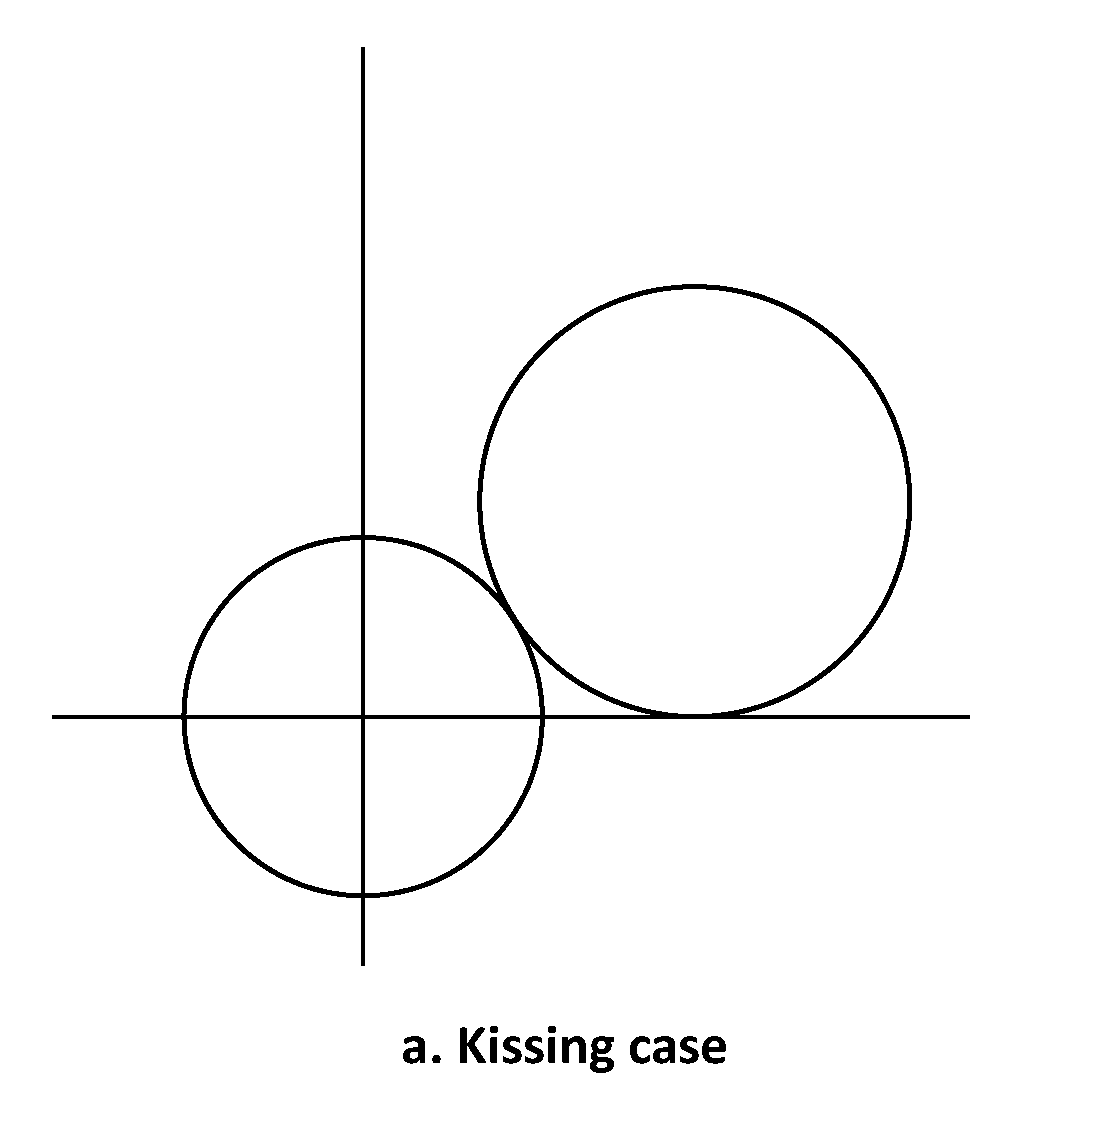
\includegraphics[height=1.65in,width=1.7in]{kissing.eps} &
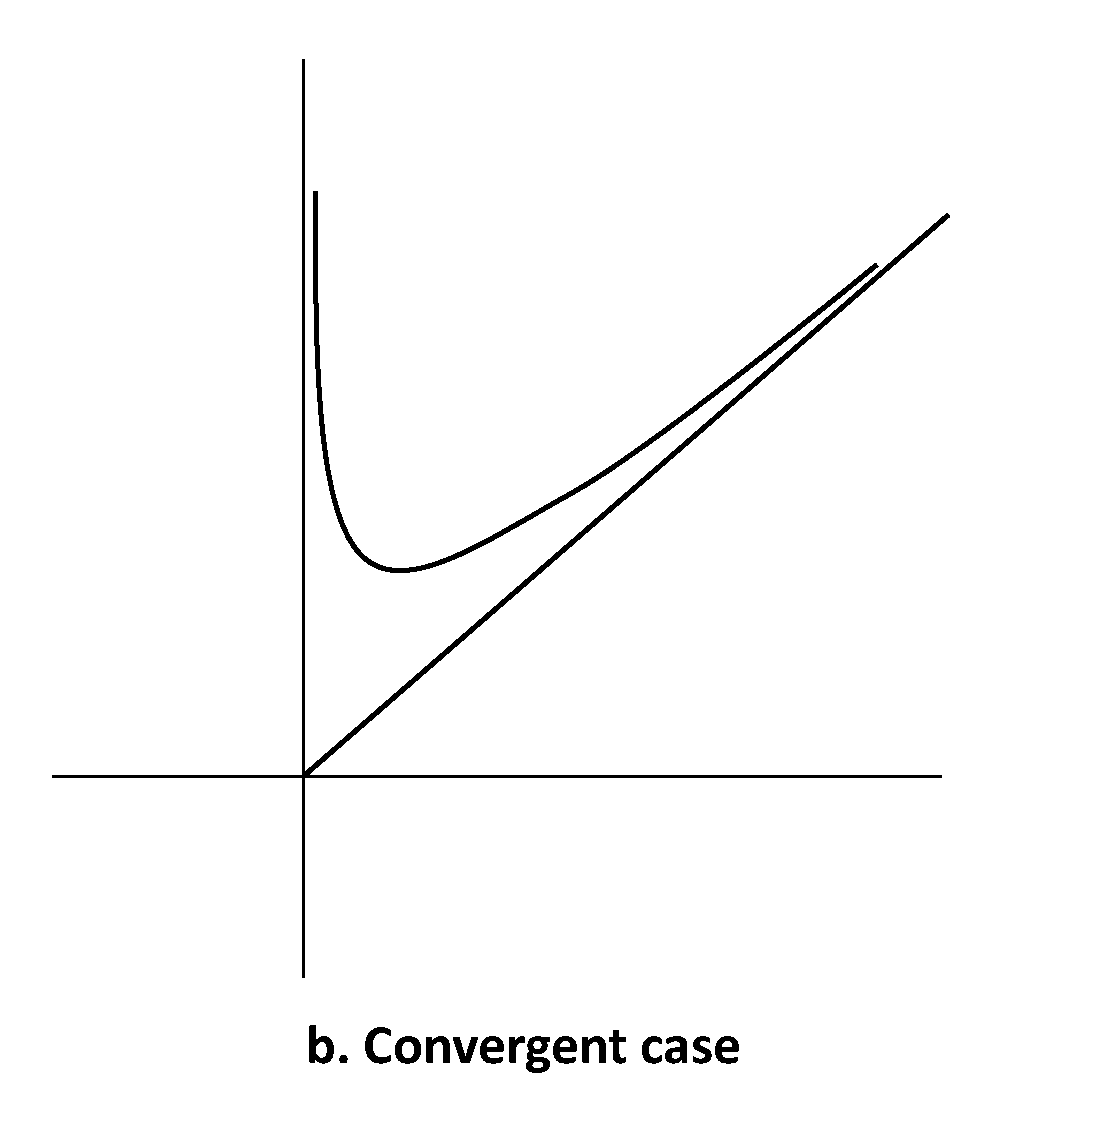
\includegraphics[height=1.65in,width=1.7in]{convergence.eps}
\end{tabular}
\caption{Limitations for proving UNSAT} 
\label{fig:limit} 
%\end{minipage}
\end{figure} 

Note that Theorem requires only $O.T$ to be converging, since $O.T$-valid works 
as $U.T$-SAT. Later in Section~\ref{sec:approximation}, we apply an interval 
arithmetic as $O.T$ (which is converging) and testing as $U.T$. 
The aims of $U.T$ are, 
\begin{itemize}
\item to accelerate SAT detection, and 
\item to guide a refinement strategy (e.g., ``First Test-UNSAT'' in 
Section~\ref{sec:intervaldecomp}). 
\end{itemize}

\section{Over and Under-Approximations for Intervals} \label{sec:approximation}

\suppress{
%From now on, we fix $F = I \wedge P$ to be a polynomial inequality such that 
%$I = x_1 \in [a_1,b_1] \wedge \cdots \wedge x_n \in [a_n,b_n]$ and 
%$P = \bigwedge \limits_{i=1}^m f_i(x_1,\cdots,x_n) > 0$. 
We present \emph{Interval Arithmetic} and \emph{Testing} as an over-approximation theory 
${O.T}$ and an under-approximation theory, ${U.T}$, respectively. 
For interval arithmetic, we apply Affine intervals (AI)~\cite{StolfiThesis} and 
Chebyshev Affine interval (CAI)~\cite{tapas12}. 

%Initially, $I$ and $P$ have conjunctions only. By refinements (decompositions of intervals), e.g., 
%$$x \in [0,2) \wedge y \in [1,3)~\mbox{to}~(x \in [0,1) \vee x \in [1.2)) \wedge (y \in [1,2) \vee y \in [2,3)),$$ 
%$I$ becomes a CNF, though $P$ has conjunctions only. 
%Thus, only $proj(I)$ is sent to a SAT solver. 
%If $P$ is a CNF, $proj(I \wedge P)$ is sent to a SAT solver, instead. 
}

\subsection{Interval Arithmetic as Over-Approximation}
A typical example of IA is Classical Interval (CI)~\cite{moore}, 
which keeps a lower bound and an upper bound. The weakness of CI is loss of dependency 
among values. For instance, if $x \in (2,4)$ then, $x - x$ is evaluated to $(-2,2)$.

Affine Interval~\cite{af,comba93} introduces \emph{noise symbols} $\epsilon$, 
which are interpreted as values in $(-1,1)$. 
For instance, $x = 3 + \epsilon$ describes $x \in (2,4)$, and 
$x - x = (3 + \epsilon) - (3 + \epsilon)$ is evaluated to $0$. 
The drawback is that the multiplication without dependency might be less precise than CI.
Affine intervals also cannot represent infinite intervals, e.g., $(0,\infty)$, 
since it becomes $\infty + \infty~\epsilon$. 
Forms of affine intervals vary by choices how to estimate multiplications. They are,
\begin{enumerate}[(i)]
\item $\epsilon \epsilon'$ is replaced with a fresh noise symbol 
($AF$)~\cite{StolfiThesis,comba93}, 
\item $\epsilon \epsilon'$ is reduced to the fixed error noise symbol 
$\epsilon_{\pm}$ ($AF_1$ and $AF_2$) \cite{af},
\item $\epsilon \epsilon'$ is replaced with $(-1,1) \epsilon$ 
(or $(-1,1) \epsilon'$) ($EAI$)~\cite{ngocsefm},
\item $\epsilon \epsilon$ is reduced to fixed noise symbols 
$\epsilon_+$ or $\epsilon_{-}$ ($AF_2$) \cite{af}, 
\item Chebyshev approximation of $x^2$ introduces a noise symbol $|\epsilon|$ 
as an absolute value of $\epsilon$ with 
$\epsilon \epsilon = |\epsilon| |\epsilon| = |\epsilon| + (-\frac{1}{4}, 0)$ and
$\epsilon |\epsilon| = \epsilon + (-\frac{1}{4}, \frac{1}{4})$ (Fig.~\ref{fig:chevabs}). 
%\item keeping products of noise symbols up to degree $2$ ($\epsilon_i \epsilon_j$),
\end{enumerate} 

\begin{figure}[ht]
\begin{minipage}[b]{1.0\linewidth}
\centering
\begin{tabular}{ll}
\includegraphics[height=1.6in,width=1.7in]{chev1.pdf} &
\includegraphics[height=1.6in,width=1.7in]{chev2.pdf}
\end{tabular}
\caption{Chebyshev approximation of $x^2$ and $x~|x|$}
\label{fig:chevabs}
\end{minipage}

\end{figure}

$CAI$ \cite{tapas12} consists of (ii) and (v), which keeps better precision than iv)
for multiplicatins of the same variables, e.g., Taylor expansion. 
%To improve precision in estimating upper and lower bounds of polynomials, we apply 
%\textbf{Affine Arithmetic} such as $AF_1$, $AF_2$ \cite{af}, $CAI$ ~\cite{tapas12} 
%instead of Classical Interval \cite{moore}. 
%Note that upper and lower bounds estimated by IA are over-approximation bounds of polynomials.

\begin{example} \label{examp:sensitivity}
Let $f = x^3 - 2xy$ with $x = (0,2)$ ($x = 1 + \epsilon_1$) and $y=(1,3)$ ($y = 2+\epsilon_2$), 
we have,
\end{example}
\begin{itemize}
\item $AF_2$ estimates the range of $f$ as 
$-3 - \epsilon_1 - 2\epsilon_2 + 3\epsilon_+ + 3\epsilon_{\pm}$, thus $(-9,6)$,
\item $CAI$ estimates the range of $f$ as 
$(-4,-\frac{11}{4}) + (-\frac{1}{4}, 0)\epsilon_1 - 2\epsilon_2 + \textbf{3}|\epsilon_1| + (-2,2)\epsilon_{\pm}$, 
thus $(-8,4.5)$.
\end{itemize}

For Affine intervals, \emph{sensitivity}~\cite{ngocsefm} of a variable
is the absolute value of the coefficient of its corresponding $\epsilon$. 
In Example~\ref{examp:sensitivity}, 
$CAI$ estimates the coefficient of $|\epsilon_1|$ as $\textbf{3}$, 
which has the largest sensitivity and indicates $x$ the most influencial. 

\suppress{
\subsection{Interval Arithmetic as Over Approximation} \label{sec:ia}
Interval arithmetic (IA) is applied for estimating bounds of polynomials 
under a given input range (a box), and 
we use it as an over-approximation theory. 
We instantiate IA to $O.T$ in Section~\ref{sec:raSATloop}, and obtain the definition below. 
}

\begin{definition}
%For $\exists x_1 \in (a_1,b_1) \cdots x_n \in (a_n,b_n). \bigwedge \limits_{i=1}^m f_i(x_1,\cdots,x_n) > 0$, 
Let $M = \bigwedge \limits_{i=1}^m x_i \in (a_i,b_i)$ and 
${\mathcal P} = \bigwedge \limits_{i=1}^m f_i(x_1,\cdots,x_n) > 0$. 
%
Let $\delta_i^l$ and $\delta_i^u$ be lower and upper bounds of $f_i(x_1,\cdots,x_n)$ 
estimated by IA for $x_i \in (a_i,b_i)$. Then, we say 
%
%\vspace*{0.5em}
\begin{itemize}
\item ${\mathcal P}$ is \emph{IA-VALID} under $M$, if IA evaluates 
$~\forall i \in [1,m].~\delta_i^l > 0$,
%\vspace*{0.33em}
\item ${\mathcal P}$ is \emph{IA-UNSAT} under $M$, 
$~\exists i \in [1,m].~\delta_i^u \leq 0$, and 
\item ${\mathcal P}$ is \emph{IA-SAT} under $M$, if 
$(\exists j \in [1,m].~\delta_j^l \leq 0)\; \wedge \; 
	(\bigwedge \limits_{i=1}^m \delta_i^u > 0)$.
\end{itemize} 
\end{definition}

IA-VALID and IA-UNSAT safely reason satisfiability (SAT) and unsatisfiability (UNSAT), 
respectively. However, IA-SAT cannot conclude SAT. 

\subsection{Testing as Under Approximation} \label{sec:test}

%We instantiate testing to $U.T$ in Section~\ref{sec:raSATloop}. 

\begin{definition}\label{def:testing}
%For $\exists x_1 \in (a_1,b_1) \cdots x_n \in (a_n,b_n). \bigwedge \limits_{i=1}^m f_i(x_1,\cdots,x_n) > 0$, 
Let $M = \bigwedge \limits_{i=1}^m x_i \in (a_i,b_i)$ and 
${\mathcal P} = \bigwedge \limits_{i=1}^m f_i(x_1,\cdots,x_n) > 0$. 
%
Let a choice function $\theta : (\Real \times \Real)^n \rightarrow \Real^n$ 
such that $\theta(M) \in (a_1,b_1) \times \cdots \times (a_n,b_n)$. 
Testing is a finite set $\Theta$ of choice functions. Then, we say 
\begin{itemize}
\item ${\mathcal P}$ is \emph{Test-SAT} under $M$ if $\theta(M)$ holds ${\mathcal P}$ 
for some $\theta \in \Theta$, and 
\item ${\mathcal P}$ is \emph{Test-UNSAT} under $M$ if $\theta(M)$ never holds ${\mathcal P}$ 
for each $\theta \in \Theta$. 
\end{itemize} 
%We denote $I \models_{test(\theta)} P$ if $\bigwedge \limits_{i=1}^m f_i(\theta(I)) > 0$ holds.
\end{definition}

%The set $\Theta$ of choice functions in definition \ref{def:testing} is a set of test data. 
Test-UNSAT does not imply UNSAT though Test-SAT implies SAT. 
We apply \emph{k-random ticks}~\cite{tapas12} as testing, which consists of periodical $k$-test instances 
with a random offset, for generating test data of each variable.
Note that we keep previously generated test data to avoid overlaps of test data. 


\section {Strategies in raSAT} \label{sec:strategy}

{\bf raSAT} loop is implemented as {\bf raSAT}, 
which uses (modified) miniSAT 2.2 as a backend SAT solver. 
Backend theories (in Section~\ref{sec:approximation}) are implementd 
in Ocaml.~\footnote{{\bf raSAT} download site at {\tt http://www.jaist.ac.jp/\~mizuhito/tools/rasat.html}}

\subsection{Strategy for Over and Under Approximations for Intervals} 

\subsubsection{UNSAT Core in Polynomial Inequality.} 
%%
\suppress{
\begin{itemize}
\item{\textbf{Very lazy theory learning rule with UNSAT cores} is applied for learning only minimal sets when $M \models_{O.T} \neg P$.}
\[
M \mathrel{\lVert} I \wedge P 
\Longrightarrow_{\textit{VL}}
\emptyset \mathrel{\lVert}  I 
\wedge (\neg l_1 \vee \cdots \vee \neg l_n ) \wedge P
\quad\textit{if}\quad
\begin{cases}
\text{$M_0=\{l_1,\ldots,l_n \} \subseteq M$,} \\
\text{$M_0$ is a minimal set and} \\
\text{$l_1 \wedge \cdots \wedge l_n \models_{O.T} \neg P$.}
\end{cases}
\]
$M_0=\{l_1,\ldots,l_n \}$ is a minimal set if and only if not existing a sub set $\{l_1,\ldots,l_k \}$ of $M_0$ such that \text{$l_1 \wedge \cdots \wedge l_k \models_{O.T} \neg P$.} 
\end{itemize}
}
%%
An UNSAT core is a minimal set $M_0 = \{ l_1, \cdots, l_n \}$ that disproves $P$ (wrt $\models_{O.T}$) 
in {\bf very lazy theory learning rule} (Section~\ref{subsec:rasatloop}). 
However, finding a precise $M_0$ is not easy, and 
we apply sound approximation of an UNSAT core $\hat{f}$ of a polynomial $f$ to obtain smaller $M_0$. 

%based on the IA-UNSAT judgment. 
%Then, $M_0$ is selected as literals in $M$ corresponding to variables in $\hat{f}$. 

\begin{definition} \label{def:unsatcore}
$\hat{f}$ is an UNSAT core of a polynomial $f$ if IA-UNSAT of  
$\hat{f} > 0$ implies IA-UNSAT of $f > 0$. 
\end{definition}

\begin{example} \label{examp: unsatcore}
Given a polynomial inequality $f=x^2 - xy - xz > 0$ with $x, y, z \in (0, \infty)$, 
$\hat{f_1} = x^2 - xy$ and $\hat{f_2} = x^2 - xz$ are two UNSAT cores of $f$.
%for $\forall x,y,z \in (0, \infty)$.
\end{example}
%%
\suppress{
For instance, $\hat{f_1} > 0$ is IA-UNSAT under $x \in (1,2) \wedge y \in (4,5)$, 
then $f > 0$ is IA-UNSAT under a set of input boxes 
$\{x\in (1,2) \wedge y \in (4,5) \wedge z \in (0,1), 
 x \in (1,2) \wedge y \in (4,5) \wedge z \in (1,2), \cdots \}$, 
which is a set of all input boxes including $x \in (1,2) \wedge y \in (4,5)$. 
For removing unsatisfiable input boxes, $\neg (x \in (1,2)) \vee \neg (y \in (4,5))$ 
is added to interval constraints $I$ as a learnt clause.
}
%%


\subsubsection{Incremental Test Data Generation} \label{sec:incremental}

The number of test data affects efficiency a lot. 
For instance, if we consider a polynomial inequality with 30 variables and we generate 
2 test data for each variable, 
we have $2^{30}$ test data as a total, which is intractable. 
The ideas for incremental test data generation are 
\begin{enumerate}
\item IA-VALID APIs are excluded, 
\item IA-SAT APIs are dynamically sorted, 
\item test data are incrementally generated during the enumeration of APIs, and 
\item discharge test data that do not satisfy previous APIs. 
\end{enumerate} 
%$P = \bigwedge \limits_{i=1}^k f_i > 0$ 

Our ideas of dynamic sorting among APIs are, 
\begin{enumerate}[(i)]
\item an API with a smaller variable set, 
\item an API that have more APIs whose variable sets are supersets, and 
\item an API with a smaller additional test data generation, 
\end{enumerate} 
have higher priority. Example~\ref{ex:inctest} in Appendix~\ref{app:IncTestEx} illustrates them. 

Let $\{ f_j > 0 \}$ be the set of IA-SAT APIs and 
let $Var(f_j)$ be the set of variables in $f_j$. 
Let 
$DEP_{f_i}=\{f_j \mid f_j \in {\mathcal P}, Var(f_i) \subseteq Var(f_j)\}$ and $dep_{f_i} = |DEP_{f_i}|$. 
An ordering $\preceq$ on $\{ f_j \}$ is given by lexicographic applications of 
$\preceq_{a}$, $\preceq_{b}$, and $\preceq_{c}$. 
%Note that $f_i \preceq f_j$ is added only when $f_i \succ f_j$ is not generated until the previous steps. 
\begin{enumerate}[(a)]
%\item $Var(f_i) \subseteq Var(f_j)$ adds $f_i \preceq f_j$. 
%\item{$Var(f_j) = Var(f_{j+1})$ implies $dep_{f_j} \leq dep_{f_{j+1}}$,}
\item $dep_{f_i} \geq dep_{f_j}$ implies $f_i \preceq_{a} f_j$. 
\item If $f_j \prec f_m$ with 
$Var(f_m) \subseteq \bigcup \limits_{f_i \succeq f_j} Var(f_i)$ and 
$Var(f_n) \nsubseteq \bigcup \limits_{f_i \succeq f_j} Var(f_i)$ is found, set $f_m \prec_{b} f_n$. 
%\item If, for some $j < m$, $Var(f_m) \subseteq \bigcup \limits_{i=1}^j Var(f_i)$ and 
%$\forall n. ~Var(f_n) \nsubseteq \bigcup \limits_{i=1}^j Var(f_i)$, then $m \leq n$, 
\item $f_i \prec f_j, f_k$ and $|Var(f_j) \setminus Var(f_i)| \leq |Var(f_k) \setminus Var(f_i)|$
imply $f_j \preceq_{c} f_k$. 
\end{enumerate}

Note that $\prec_{b}$ may violate the anti-symmetry. {\bf raSAT} finds $\preceq$ by a procedure, 
and if $f_i \prec_{b} f_j$ has set in advance, it will not set $f_j \prec_{b} f_i$. 
We intend that 
(a) for (i), (ii) (since $Var(f_i) \subseteq Var(f_j)$ implies $dep_{f_i} \geq dep_{f_j}$), and 
(b), (c) for (iii). 

An ordering $\preceq$ may be partial, and {\bf raSAT} randomly fulfills it to be total. 
Then, it renumbers the indecies such that $f_1 \prec f_2 \prec \cdots$. 
Test data are incrementally generated during this enumeration, i.e., generate test data 
for $Var(f_1)$, $Var(f_2)$, and so far. 
During the enumeration, test data that failed previous APIs are removed. 
When they become empty, it reports Test-UNSAT. 
%{\bf raSAT} loop moves to the refinement phase. 



\subsection{Interval Refinements} \label{sec:refinement}

\suppress{
We need to consider the choice of intervals to decompose, and 
how to decompose an interval. 
Similar to explosion of test data generation, interval decomposition may cause exponential 
explosion of boxes. 
Certain strategies to choose variables to apply interval decompositions, and 
how to decompose intervals are crucial in practice. 
}

\medskip
\subsubsection{Selecting Intervals to Refine}  \label{sec:intervaldecomp}

Refinement shares the same explosion problem with test data generation. 
The choice of intervals to refine has two steps. 
\begin{enumerate}[(a)]
\item Choose an API such that its variables are candidates for refinements. 
\item Among variables, choose influential ones. 
\end{enumerate}

(a) follows incremental test data generation in Section~\ref{sec:incremental}. 
When an API $f_j > 0$ refutes all generated test data, it returns Test-UNSAT. 
Then, variables appearing in $f_j$ are candidates for refinement, 
since $f_j$ is a direct cause of Test-UNSAT. In Example~\ref{ex:inctest}, 
Test-UNSAT of $2yv^2 - ux^2 - 1 > 0$ is reported with $\{v=0.7, v=1.3\}$, 
and $x,y,u,v \in (0,2)$ become candidates for refinement. 

For (b), among variables in the candidate API $f_j > 0$, we further filter variables that 
have larger sensitivity (Example~\ref{examp:sensitivity}), since they are expected to be more 
influential. Sensitivity is detected by previous IA-SAT detection phase. 
Among presented strategies, only this step is not implemented in current {\bf raSAT}.

\medskip
\subsubsection{Interval Decomposition} \label{subsec:decomposition}

The first choice of interval decomposition is a {\em Balanced decomposition}, 
which exactly decomposes an interval into half and half. 
%%
\suppress{
%\smallHead{Balanced Decomposition} \label{sec:balanced}
 decomposes an interval into two intervals exactly half. 

\begin{definition}
For an interval $x \in (a,b)$, a balanced decomposition is 
\[
D_b(x\in(a,b)) = \{x \in (a, \frac{a+b}{2}), x \in (\frac{a+b}{2}, b)\} 
\]
\end{definition} 
}
%%
%\smallHead{Monotonic Decomposition.} \label{sec:unbalanced}
Instead, we adopt {\em monotonic decomposition}, which introduces bias $\delta$ 
when a value of a corresponding variable monotonically affects to that of a polynomial. 

\begin{definition} \label{def:mono}
Let $f(x_1, \cdots,x_k)$ be a polynomial, a variable $x_i$ is monotonic (resp. anti-monotonic) in $f$ 
if $x_i' \geq x_i''$ implies $f(\cdots,x_i',\cdots) \geq f(\cdots,x_i'',\cdots)$ 
(resp. $f(\cdots,x_i',\cdots) \leq f(\cdots,x_i'',\cdots)$).
$Pos_f$ (resp. $Neg_f$) denotes the set of monotonic (resp. anti-monotonic) variables in $f$. 

Then, a monotonic decomposition on $x \in (a,b)$ with $\delta < b-a$ is, 
\[
\begin{cases}
\{x\in (a,b-\delta), x \in (b-\delta,b)\} & \textit{if} ~x \in Pos_f\\
\{x\in (a,a+\delta), x \in (a+\delta,b)\} & \textit{if} ~x \in Neg_f\\
\{x \in (a, \frac{a+b}{2}), x \in (\frac{a+b}{2}, b)\} & \textit{otherwise}\\
\end {cases}
\]
%two sets of monotone variables $Pos_f$, $Neg_f$, 
\end{definition} 

The bias $\delta$ in Definition~\ref{def:mono} is shared with $\delta$ in Definition~\ref{def:ishalt}. 
%For a balanced decomposition, SAT solver will choose an arbitrary combination of input ranges. 
As a choice of SAT instances, we hope to force SAT solver to choose a narrower sub interval 
(i.e., $(b-\delta,b)$ for $Pos_f$, and $(a, a+\delta)$ for $Neg_f$), 
which would make bounds of $f$ approaching, and provide more chances to lead $f$ satisfiable.
% The choices are $(h-\delta, h)$  and either $(l, \frac{h+l}{2})$ or $(\frac{h+l}{2}, h)$ for remaining.
MiniSAT 2.2 decides it by the ``activity'' measure, and we modify that part in MiniSAT 2.2. 

\begin{figure}[ht]
\centering
\begin{minipage}[b]{0.45\linewidth}
  \includegraphics[height=1.8in,width=1.9in]{interval_dec.eps}
\caption{Interval decompositions}
\label{fig:decomposition}
\end{minipage}
\quad
\begin{minipage}[b]{0.45\linewidth}
\includegraphics[height=2in,width=2in]{equality.eps}
\caption{Intermediate Value Theorem}
\label{fig:ivt}
\end{minipage}
\end{figure}

%\begin{figure}
%\begin{center}
  %\includegraphics[height=2in,width=2in]{equality.eps}
%\end{center}
%\caption{Intermediate Value Theorem}
%\label{fig:ivt}
%\end{figure}


\section{Equality handling} \label{sec:equality}

\subsection{Greater-than-or-Equal Handling} \label{sec:geq}

{\bf raSAT} loop is designed to solve polynomial inequality. 
There are several ways to extend to handle equality, in which our idea shares similarity with 
dReal~\cite{dRealCADE13,dRealLICS12}. 

\begin{definition} \label{def:strict_unsat}
$\bigwedge \limits_{j} f_j \geq 0$ is 
{\em strict-SAT} (resp. {\em strict-UNSAT}) 
if $\bigwedge \limits_{j} f_j > \delta_j$ is SAT 
(resp. $\bigwedge \limits_{j} f_j > -\delta_j$ is UNSAT) for some $\delta_j >0$.
\end{definition}

\begin{lemma} \label{lem:strict_sat}
If $\bigwedge \limits_{j} f_j \geq 0$ is {\em strict-SAT} (resp. {\em strict-UNSAT}), 
it is SAT (resp. UNSAT).
\end{lemma}

Note that netiher strict-SAT nor strict-UNSAT (i.e., kissing situation), 
%if $\bigwedge \limits_{j} f_j \geq 0$ is SAT but $\bigwedge \limits_{j} f_j > 0$ is UNSAT 
Lemma~\ref{lem:strict_sat} cannot conclude anything, and \textbf{raSAT} says {\em unknown}. 
%In implementation of \textbf{raSAT}, when $\geq$ appears, exploration of IA-SAT 
%(resp. IA-UNSAT) is reduced to that of IA-strict-SAT (resp. IA-strict-UNSAT). 


\subsection{SAT on Equality by Intermediate Value Theorem} \label{sec:eq}
For solving polynomial constraints with single equality ($g=0$), we apply {\em Intermediate Value Theorem}. 
That is, if existing 2 test cases such that $g > 0$ and $g < 0$, then $g=0$ is SAT somewhere in between, 
as in Fig.~\ref{fig:ivt}. 

\begin{lemma} \label{lemma:ivt}
For $F = \exists x_1 \in (a_1,b_1) \wedge \cdots \wedge x_n \in (a_n,b_n). 
\bigwedge \limits_{j}^m f_j > 0~\wedge~g = 0$, $F$ is SAT, if 
there is a box $(l_1, h_1) \times \cdots \times (l_n,h_n)$ with $ (l_i,h_i) \subseteq (a_i,b_i)$ 
such that 
\begin{enumerate}[(i)]
\item $\bigwedge \limits_{j}^m f_j > 0$ is IA-VALID in the box, and 
\item there are two instances $\vec{t},\vec{t'}$ in the box with $g(\vec{t}) > 0$ and $g(\vec{t'}) < 0$.
\end{enumerate}
\end{lemma}

{\bf raSAT} first tries to find an IA-VALID box for $\bigwedge \limits_{j}^m f_j > 0$ by refinements. 
If such a box is found, it tries to find 2 instances for $g > 0$ and $g < 0$ by testing. 
Intermediate Value Theorem guarantees the existence of an SAT instance in between. 
Note that this method works for single equality and does not find an exact SAT instance. 
If multiple equalities do not share variables each other, we can apply Intermediate Value Theorem 
repeatedly to decide SAT. In Zankl benchmarks in SMT-lib, there are 15 gen-**.smt2 that contain equality
(among 166 problems), and each of them satisty this condition. 


 
\suppress{
In Table \ref{tab:eqexp} we show preliminary experiment for 15 problems that contain polynomial equalities in Zankl family. \textbf{raSAT} works well for these SAT problems and it can detect all SAT problems (11 among 15). At the current implementation, raSAT reports \emph{unknown} for UNSAT problems. The first 4 columns indicate \emph{name of problems}, \emph{the number of variables}, \emph{the number of polynomial equalities} and \emph{the number of inequalities}  in each problem, respectively. The last 2 columns show comparison results of \textbf{Z3 4.3} and \textbf{raSAT}.
\begin{table}
\centering
\scalebox{1.0}{
\begin{tabular}[b]{|c|c|c|c|c|c|c|c|}
\hline
%\multirow{2}{*}{Problem} & {No.} & {No.} & {No.}&
{Problem} & {No.} & {No.} & {No.}&
\multicolumn{2}{c|}{\textbf{Z3 4.3} (15/15)} &\multicolumn{2}{c|}{\textbf{raSAT} (11/15)}\\
\cline{5-8}
Name & Variables& Equalities& Inequalities&{Result} & {Time(s)}&{Result} & {Time(s)}\\
\hline
gen-03 & 1 & 1 & 0& SAT &0.01 & SAT &0.015\\
\hline
gen-04 & 1 & 1 & 0& SAT &0.01 & SAT &0.015\\
\hline
gen-05 & 2 & 2 & 0& SAT &0.01 & SAT &0.046\\
\hline
gen-06 & 2 & 2 & 1& SAT &0.01 & SAT &0.062\\
\hline
gen-07 & 2 & 2 & 0& SAT &0.01 & SAT &0.062\\
\hline
gen-08 & 2 & 2 & 1& SAT &0.01 & SAT &0.062\\
\hline
gen-09 & 2 & 2 & 1& SAT &0.03 & SAT &0.062\\
\hline
gen-10 & 1 & 1 & 0& SAT &0.02 & SAT &0.031\\
\hline
gen-13 & 1 & 1 & 0& UNSAT &0.05 & unknown &0.015\\
\hline
gen-14 & 1 & 1 & 0& UNSAT &0.01 & unknown &0.015\\
\hline
gen-15 & 2 & 3 & 0& UNSAT &0.01 & unknown &0.015\\
\hline
gen-16 & 2 & 2 & 1& SAT &0.01 & SAT &0.062\\
\hline
gen-17 & 2 & 3 & 0& UNSAT &0.01 & unknown &0.031\\
\hline
gen-18 & 2 & 2 & 1& SAT &0.01 & SAT &0.078\\
\hline
gen-19 & 2 & 2 & 1& SAT &0.05 & SAT &0.046\\
\hline
\end{tabular}
}
\caption{Experimental results for 15 equality problems of Zankl family}
\label{tab:eqexp}
\end{table}

We also apply the same idea for multiple equalities $\bigwedge \limits_{i} g_i = 0$ such that $Var(g_k) \cap Var(g_{k'}) = \emptyset$ where $Var(g_k)$ is denoted for the set of variables in the polynomial $g_k$. In the next section we will present idea for solving general cases of multiple equalities.
}



\section{Experiments} \label{sec:experiment}

%\subsection{{\bf raSAT} Implementation} 
We implement \textbf{raSAT} loop as an SMT {\bf raSAT}, 
based on MiniSat 2.2 as a backend SAT solver. 
We will compare {\bf raSAT} with \textbf{Z3 4.3} (the latest version), 
since Table.1 in~\cite{Jovanovic13} shows the strength of \textbf{nlSAT}
(equivalently, Z3 4.3). 
Note that our comparison is only on polynomial inequality. 
Example~\ref{ex1} in Appendix~\ref{app:raSATexample} illustrates how {\bf raSAT} works. 


\suppress{
Z3 (version 3.1) is the winner of SMT competition 2011 for QF\_NRA and the 
latest version (\textbf{Z3 4.3}) is also called by another name \textbf{nlSAT} 
\cite{Jovanovic13}, which is known as a very strong SMT solver for non-linear arithmetic. 
%CVC3 \cite{cvc3} participated in SMT competition 2010 and 2011 too.
}
We apply \emph{2-random ticks} for testing, \emph{Test-UNSAT} of testing and 
\emph{monotonic decomposition} for refinements. In these experiments, 
we do not include UNSAT core and sensitivity strategy, which are not implemented yet. 
All tests are run on a system with Intel Core Duo L7500 1.6 GHz and 2 GB of RAM.

\suppress{
It chooses a combination of input ranges for all variables, which is first evaluated by IA. 
If IA informs IA-UNSAT, \emph{very lazy theory learning rule} is applied
and it chooses another combination of input ranges. 
If IA informs IA-VALID, {\bf raSAT} terminates and outputs SAT. Otherwise, testing is applied. 

Testing generates test data from a given combination of input ranges. 
Testing will stop when it results Test-SAT, i.e., a SAT solution is found, or 
it finds the set of Test-UNSAT APIs. 
They are sent to \emph{interval decomposition} and a refinement rule is applied. 

If all input ranges become small enough, heuristic rule is applied. 
Once heuristic rules are used, {\bf raSAT} concludes \emph{unknown} when the SAT solver 
informs UNSAT. 
If they are never used, {\bf raSAT} concludes UNSAT when the same occurs. 
We apply various \emph{affine intervals} for IA and \emph{k-random ticks} for testing. 

\begin{figure}
\centering
  \includegraphics[height=2.7in,width=2.8in]{framework.eps}
\caption{Framework of the SMT solver \textbf{raSAT}}
\label{fig:frame}
\end{figure}
}



\subsection {Preliminary Evaluation} \label{sec:experiments}
There are three immediate measures on the size of polynomial constraints. They are the highest degree of polynomials, the number of variables, and the number of APIs. We prepare simple benchmarks focusing on these measures. 

For the first and the second measures, we apply 
\begin{equation}\label{eq:circle}
\psi = \displaystyle \sum\limits_{i=1}^{k} x_i^n < 1 \wedge 
\displaystyle \sum\limits_{i=1}^{k} (x_i-r)^n < 1
\end{equation} 

For experiments on these problems, 
To make SAT and UNSAT problems, we adjust values of $r$ around the threshold 
$\sqrt[n]{\frac{1}{k}}$ (for fixed $k$ and $n$), which separates SAT and UNSAT. 
%Figure \ref{fig:far} and \ref{fig:close} demonstrate the choices of $r$. 
In our experiments we choose values of $r$ with $|r - \sqrt[n]{\frac{1}{k}}| < 0.01$.

%For settings of \textbf{raSAT}, 
For termination heuristics $isHalt$, $\delta$ is set to $0.005$, and 
the initial interval constraints are $\bigwedge \limits_{i} x_i \in (-1,1)$.

%Note that \textbf{CVC3 2.4.1} reports \emph{unknown} for all problems in three measures, 
%thus we only show results of \textbf{raSAT} and \textbf{Z3 4.3}.




\smallHead{The degree of polynomials}

Table~\ref{tab:expdegree} shows results of \textbf{raSAT} and \textbf{Z3 4.3} 
for the problems $\psi = x_1^n + x_2^n < 1 \wedge (x_1-r)^n + (x_2-r)^n <1$
with $k=2$, $n = 8, 10, 12,..., 22$. 
%The results are shown in Tab.~\ref{tab:expdegree}. 
The first column indicates whether SAT or UNSAT, followed by the columns of $k$, $n$ and $r$. 
Running time (in seconds) of \textbf{Z3 4.3} and \textbf{raSAT} are in the last two columns. 
For the degree 22, the results of \textbf{Z3 4.3} are $''? >3600''$, which means 
that \textbf{Z3 4.3} cannot finish in 3600 seconds. 
{\bf raSAT} outperforms \textbf{Z3 4.3}, and this is not surprising since IA and testing are 
not affected much by the increase of degrees. 

\begin{table}
\centering
\scalebox{1.0}{
\begin{tabular}[b]{|c|c|c|c|r|r|}
\hline
\multirow{2}{*}{SAT/UNSAT} & \multirow{2}{*}{k} & \multirow{2}{*}{n} & \multirow{2}{*}{r}&
\multicolumn{2}{c|}{Time(s)} \\
\cline{5-6}
& & & & {Z3 4.3} & {raSAT}\\
\hline
SAT & 2 & 8 & 1.83& 1.330 &0.265 \\
\hline
UNSAT & 2 & 8 & 1.84& 0.580 &0.328 \\
\hline
SAT & 2 & 10 & 1.86 & 4.530& 0.140\\
\hline
UNSAT & 2 & 10 & 1.87 & 125.000& 0.796\\
\hline
SAT & 2 & 12 & 1.88& 0.360& 0.140\\
\hline
UNSAT & 2 & 12 & 1.89& 40.280& 1.390\\
\hline
SAT & 2 & 14 & 1.90& 0.480& 0.296\\
\hline
UNSAT & 2 & 14 & 1.91& 78.730& 0.531\\
\hline
SAT & 2 & 16 & 1.91& 2.250& 0.109\\
\hline
UNSAT & 2 & 16 & 1.92& 174.000& 0.484\\
\hline
SAT & 2 & 18 & 1.92& 289.110& 0.562\\
\hline
UNSAT & 2 & 18 & 1.93& 391.670& 0.765\\
\hline
SAT & 2 & 20 & 1.93& 1259.560& 1.468\\
\hline
UNSAT & 2 & 20 & 1.94& 1650.860& 0.921\\
\hline
SAT & 2 & 22 & 1.93& $? >3600$& 0.437\\
\hline
UNSAT & 2 & 22 & 1.94& $? >3600$& 3.203\\
\hline
\end{tabular}
}
\caption{Experimental results for $\psi = x_1^n + x_2^n < 1 \wedge (x_1-r)^n + (x_2-r)^n <1$}
\label{tab:expdegree}
\end{table}



\smallHead{The number of variables}

We set simple benchmarks by instantiating $k=3,4,5,6$ and $n=4,6,8$ 
to the formula~\ref{eq:circle}. 
{\bf raSAT} loop decomposes boxes, and the number of boxes can easily grow 
exponentially. To hold down it in practice, we introduce a strategy to 
select an API in which each variable is applied an interval decomposition
(Section~\ref{sec:refinement}). 
Here, the timeout is set to $600$ seconds for each problem, 
and the results is shown in Table~\ref{tab:expvar}, which show that 
the selection strategy seems working well. 

\begin{table}
\centering
\scalebox{1.0}{
\begin{tabular}[b]{|c|c|c|c|r|r|}
\hline
\multirow{2}{*}{SAT/UNSAT} & \multirow{2}{*}{k} & \multirow{2}{*}{n} & \multirow{2}{*}{r}&
\multicolumn{2}{c|}{Time(s)} \\
\cline{5-6}
& & & & {Z3 4.3} & {raSAT}\\
\hline
SAT & 3 & 4 & 1.51& 0.030 &0.027 \\
\hline
UNSAT & 3 & 4 & 1.52& 10.560 & \footnotesize{\emph{timeout}}\\
\hline
SAT & 4 & 4 & 1.41 & \footnotesize{\emph{timeout}}& 0.390\\
\hline
UNSAT & 4 & 4 & 1.42 & \footnotesize{\emph{timeout}}& \footnotesize{\emph{timeout}}\\
\hline
SAT & 5 & 4 & 1.33& \footnotesize{\emph{timeout}}& 51.578\\
\hline
UNSAT & 5 & 4 & 1.34& \footnotesize{\emph{timeout}}& \footnotesize{\emph{timeout}}\\
\hline
SAT & 6 & 4 & 1.27& \footnotesize{\emph{timeout}}& 111.031\\
\hline
UNSAT & 6 & 4 & 1.28& \footnotesize{\emph{timeout}}& \footnotesize{\emph{timeout}}\\
\hline
SAT & 3 & 6 & 1.66& \footnotesize{\emph{timeout}} &0.890 \\
\hline
UNSAT & 3 & 6 & 1.67& \footnotesize{\emph{timeout}} &62.765 \\
\hline
SAT & 4 & 6 & 1.58 & \footnotesize{\emph{timeout}}& 1.156\\
\hline
UNSAT & 4 & 6 & 1.59 & \footnotesize{\emph{timeout}}& \footnotesize{\emph{timeout}}\\
\hline
SAT & 5 & 6 & 1.52& \footnotesize{\emph{timeout}}& 73.937\\
\hline
UNSAT & 5 & 6 & 1.53& \footnotesize{\emph{timeout}}& \footnotesize{\emph{timeout}}\\
\hline
SAT & 6 & 6 & 1.48& \footnotesize{\emph{timeout}}& 239.968\\
\hline
UNSAT & 6 & 6 & 1.49& \footnotesize{\emph{timeout}}& \footnotesize{\emph{timeout}}\\
\hline
SAT & 3 & 8 & 1.74& \footnotesize{\emph{timeout}}& 3.125\\
\hline
UNSAT & 3 & 8 & 1.75& \footnotesize{\emph{timeout}}& 37.156\\
\hline
SAT & 4 & 8 & 1.68& \footnotesize{\emph{timeout}}& 69.843\\
\hline
UNSAT & 4 & 8 & 1.69& \footnotesize{\emph{timeout}}& \footnotesize{\emph{timeout}}\\
\hline
\end{tabular}
}
\caption{Experimental results for 
$\psi = \displaystyle \sum\limits_{i=1}^{k} x_i^n < 1 \wedge 
	\displaystyle \sum\limits_{i=1}^{k} (x_i-r)^n < 1$}
\label{tab:expvar}
\end{table}


\smallHead{The number of APIs}

Simple benchmarks to measure the effect of the number of APIs are prepared as
the formula $\psi = \psi_1 \wedge \psi_2$ where,
\begin{itemize}
\item $\psi_1 = x_0^n + x_1^n< 1 \wedge x_1^n + x_2^n< 1 \wedge \cdots \wedge x_k^n + x_0^n< 1$
\item $\psi_2 = (x_0-r)^n + (x_1-r)^n < 1 \wedge (x_1-r)^n + (x_2-r)^n < 1 
	\wedge \cdots \wedge (x_k-r)^n + (x_0-r)^n < 1$
\end{itemize}
We fixed $n=6$ and $k$ is from $3$ to $15$. 
The timeout is set by $600$ seconds and $|r - \sqrt[n]{\frac{1}{2}}| < 0.01$.
The results are shown in Table~\ref{tab:expapi}. Generally, {\bf raSAT} shows better 
results than Z3 4.3. 

\begin{table}
\centering
\scalebox{1.0}{
\begin{tabular}[b]{|c|c|c|c|r|r|}
\hline
\multirow{2}{*}{SAT/UNSAT} & \multirow{2}{*}{k} & \multirow{2}{*}{n} & \multirow{2}{*}{r}&
\multicolumn{2}{c|}{Time(s)} \\
\cline{5-6}
& & & & {Z3 4.3} & {raSAT}\\
\hline
%SAT & 2 & 6 & 1.78& 0.050 &0.093 \\
%\hline
%UNSAT & 2 & 6 & 1.79& 0.690 &0.375 \\
%\hline
SAT & 3 & 6 & 1.78 & \footnotesize{\emph{timeout}}& 0.171\\
\hline
UNSAT & 3 & 6 & 1.79 & 0.280& 0.796\\
\hline
%SAT & 4 & 6 & 1.78& 0.080& 0.453\\
%\hline
%UNSAT & 4 & 6 & 1.79& 0.280& 0.671\\
%\hline
SAT & 5 & 6 & 1.78& \footnotesize{\emph{timeout}}& 0.375\\
\hline
UNSAT & 5 & 6 & 1.79& 0.280& 0.640\\
\hline
%SAT & 6 & 6 & 1.78& 0.050& 0.609\\
%\hline
%UNSAT & 6 & 6 & 1.79& 0.220& 1.203\\
%\hline
SAT & 7 & 6 & 1.78& \footnotesize{\emph{timeout}}& 0.765\\
\hline
UNSAT & 7 & 6 & 1.79& 0.250& 0.734\\
\hline
%SAT & 8 & 6 & 1.78& 0.050& 2.015\\
%\hline
%UNSAT & 8 & 6 & 1.79& 0.230& 1.468\\
%\hline
SAT & 9 & 6 & 1.78& \footnotesize{\emph{timeout}}& 2.671\\
\hline
UNSAT & 9 & 6 & 1.79& 0.300& 1.921\\
\hline
SAT & 11 & 6 & 1.78& \footnotesize{\emph{timeout}}& 3.328\\
\hline
UNSAT & 11 & 6 & 1.79& 0.220& 1.343\\
\hline
SAT & 13 & 6 & 1.78& \footnotesize{\emph{timeout}}& 4.460\\
\hline
UNSAT & 13 & 6 & 1.79& 0.300& 1.875\\
\hline
SAT & 15 & 6 & 1.78& \footnotesize{\emph{timeout}}& 6.640\\
\hline
UNSAT & 15 & 6 & 1.79& 0.300& 2.265\\
\hline
\end{tabular}
}
\caption{Experimental results for $\psi = \psi_1 \wedge \psi_2$}
\label{tab:expapi}
\end{table}

\suppress{
In the experiments from simple benchmarks for three measures above, \textbf{raSAT} outperforms \textbf{Z3 4.3} and we have some observations, which are,
\begin{itemize}
\item \textbf{Z3 4.3} meets difficulties for high degree problems, i.e., problems of 2 variables with degrees 20, 22, and problems of 4, 5 variables with degrees 4, 6, 8 in these experiments,

\item \textbf{raSAT} works quite well for high degrees and increasing number of APIs. It reports results \emph{very fast} in comparison with \textbf{Z3 4.3}.

\item However \textbf{raSAT} suffers from enlarging dimensions for both SAT and UNSAT problems. We need further comparison, investigation, and reasonable strategies for increasing dimensions because explosion of boxes occurs when intervals are decomposed in \textbf{raSAT}.
\end{itemize}
}

\subsection{Benchmarks from SMT-LIB} \label{sec:expsmtlib}

In SMT-LIB~\footnote{\tt http://www.smt-lib.org}, 
benchmark programs on non-linear real number arithmetic 
(QF\_NRA) are categorized into Meti-Tarski, Keymaera, Kissing, Hong, and Zankl families. 
Until SMT-COMP 2011, benchmarks are only Zankl family. 
In SMT-COMP 2012, other families have been added, and currently growing. 
General comparison among various existing tools on these benchmarks is summarized in 
Table.1 in \cite{Jovanovic13}, which shows Z3 4.3 is one of the strongest. 

\begin{table*}[t]
\centering
\scalebox{1.15}{
{\renewcommand{\arraystretch}{1.3}
\begin{tabular}{|l|c|c|r|c|c|r|c|c|r|}
\hline
\multirow{2}{*}{Solver} & \multicolumn{3}{c|}{Hong (20)} & \multicolumn{3}{c|}{Zankl (151)} & \multicolumn{3}{c|}{Meti-Tarski (832)}\\
\cline{2-10}
& {SAT} &{UNSAT}  &{time(s)} & {SAT} & {UNSAT}  &{time(s)} & {SAT} & {UNSAT}  &{time(s)}\\
%\hline
%{CVC3 2.4.1} & 0 & 0 & 0 & 0 & 9 &10.678 & -- & -- & --\\
\hline
\textbf{Z3 4.3}& 0& 8 & 5.620 & \textbf{50} &\textbf{24}& \textbf{1144.320} & \textbf{502} & \textbf{330} & \textbf{33.350} \\
\hline
\textbf{raSAT} & 0& \textbf{20} & 381.531 & 42 &9 & 2417.931 & 501 & 156 & 21.989\\
\hline
\end{tabular}
}
}
\medskip
\caption{Experimental results for Hong, Zankl, and Meti-Tarski families}
\label{tab:expsmtlib}
\end{table*}

From them, we take problems of polynomial inequality only %(not containing $''=''$). 
The brief statistics and explanation are as follows. 
\begin{itemize}
\item {\bf Meti-Tarski} contains 5364 inequalities among 8377, taken from elementary physics.
Typically, they are small problems which have lower degrees and few variables, 
i.e., 3 or 4 variables in each problem. 
Frequently, linear constraints are mixed in these problems.
\item {\bf Keymaera} contains 161 inequalities among 4442. 
\item {\bf Kissing} has 45 problems, all of which contains equality (mostly single equality). 
%They are taken from the cases of touching curves. 
\item {\bf Hong} has 20 inequalities among 20, tuned for QE-CAD and quite artificial. 
\item {\bf Zankl} has 151 inequalities among 166, taken from termination provers. 
Problems may contain many ($>100$) variables, in which some APIs have $>15$ variables
\end{itemize}


We perform experiments only on Hong, Zankl, and Meti-Tarski families. 
Table \ref{tab:expsmtlib} shows the number of solved problems and 
their total running time (in seconds). 

Among 20 problems of Hong family, their degrees distribute from 1 to 20. 
{\bf raSAT} solved all of them (all are UNSAT). {\bf Z3 4.3} solved 8 problems, 
whose degrees are up to 8. 
%{\bf Z3 4.3} becomes timeout for other problems, which have higher degrees than 8. 
Note that iSAT can also solve all of problems in Hong family. 

For Zankl family,  {\bf Z3 4.3} shows better performance than {\bf raSAT}. 
 {\bf Z3 4.3} runs very fast for problems that contain linear constraints combined with 
non-linear constraints of lower degrees (e.g., degree $4$). 
We observe that {\bf raSAT} outperforms {\bf Z3 4.3} when problems have 
a long monomial (e.g., 60), higher degrees (e.g., 6), and APIs with more variables 
(e.g., $>14$). 
For instance, only {\bf raSAT} can solve \emph{matrix-2-all-5,8,11,12}, and 
is quicker to show SAT (by testing) in \emph{matrix-2-all-9,10}. 

Among large number of problems in Meti-Tarski, 
we extract 832 problems for the experiment. 
\textbf{Z3 4.3} solved all problems, and 
\textbf{raSAT} solved 657 (SAT/UNSAT) problems among 832. 
Actually, \textbf{raSAT} solved almost all SAT problems, 
but UNSAT problems are less. 
One reason is that kissing cases occur frequently in UNSAT problems of Meti-Tarski, 
which \textbf{raSAT} cannot handle. 
%We expect that preprocessing on linear constraint parts could improve. 
Note that, in Table.1 in \cite{Jovanovic13}, only QE-CAD based tools work fine 
(\textbf{Z3 3.1} does not apply QE-CAD, whereas \textbf{Z3 4.3} $=$ \textbf{nlSAT}
includes QE-CAD). 
Although \textbf{raSAT} has certain limitations on UNSAT problems, 
it shows enough comparable results in Meti-Tarski benchmarks 
and seems faster than most of QE-CAD based tools (except for \textbf{Z3 4.3}). 


\suppress{
Its results are interesting,
\begin{itemize}
\item almost SAT problems are detected by \textbf{raSAT},
\item total running time of \textbf{raSAT} is impressive, 
i.e., 657 problems are solved in 22 seconds,
\item as showing in Table.1 in \cite{Jovanovic13}, 
QE-CAD approach shows strong results for Meti-Tarski problems, 
others are quite weak. However, \textbf{raSAT} shows competitive results.
\end{itemize}
}

%\begin{table}
%\centering
%\scalebox{0.85}{
%\begin{tabular}[b]{|c|c|c|c|c|c|}
%\hline
%{Timeout setting (s)}& {\textbf{Solvers}} & {\textbf{SAT}}  &{\textbf{UNSAT}} & {\textbf{unknown}} &
%{\textbf{Timeout}} \\
%\hline
%\multirow{3}{*} {900} & {\textbf{CVC3 2.4.1}}& 0 & 0 & 20 & 0\\
%& \textbf{Z3 4.3}& 0 & 10 & 0 & 10\\
%& {\textbf{RASMT}} & 0 & 20 & 0 & 0\\
%\hline
%\multirow{3}{*} {300} & {\textbf{CVC3 2.4.1}}& 0 & 0 & 20 & 0\\
%& \textbf{Z3 4.3}& 0 & 10 & 0 & 10\\
%& {\textbf{RASMT}} & 0 & 20 & 0 & 0\\
%\hline
%\end{tabular}
%}
%\caption{Experimental results for \textbf{Zankl} family}
%\label{tab:zankl}
%\end{table}




\section{Conclusion} \label{sec:conclusion and Future Work}


This paper presented {\bf raSAT} loop, which mutually refines over and under--approximation 
theories. For polynomial inequlaity, we adopted interval arithemtic and testing for 
over and under-approximation theories, respectively. 
{\bf raSAT} loop is implemented as an SMT {\bf raSAT}. 
The result of Experiments on QF\_NRA in SMT-lib is encouraging, and 
{\bf raSAT} shows comparable and sometimes outperforming to existing SMTs, e.g., 
Z3 4.3, HySAT, and dReal. For instance, ****** which has ** variables and degree ** 
was solved by {\bf raSAT}, whereas none of above mentioned SMTS can. 
%
\suppress{
\subsection{Observation and Discussion} 

From experimental results in Section~\ref{sec:experiments} and~\ref{sec:expsmtlib}, 
we observe the followings. 
\begin{itemize}
\item The degree of polynomials will not affect much. 
\item The number of variables are matters, but also for Z3 4.3. 
The experimental results do not show exponential growth, and we expect 
the strategy of selection of an API in which related intervals are decomposed
seems effective in practice. By observing Zankl examples, we think the maximum 
number of variables of each API seems a dominant factor. 
\item Effects of the number of APIs are not clear at the moment. In simple benchmarks, 
{\bf raSAT} is faster than Z3 4.3, however we admit that we have set small degree $n=6$
for each API. 
\end{itemize}

For instance, {\em matrix-2-all-5,8,11,12} in Zankl 
contain a long monomial (e.g., $60$) with the max degree $6$, and 
relatively many variables (e.g., $14$), which cannot be solved by Z3 4.3, but 
{\bf raSAT} does. 
As a general feeling, if an API contains more than $30 \sim 40$ variables, 
{\bf raSAT} seems saturating. 
We expect that, adding to a strategy to select an API (Section~\ref{sec:intervaldecomp}), 
we need a strategy to select variables in the focus. We expect this can be designed 
with sensitivity (Example~\ref{examp:sensitivity}) and would work in practice. 
Note that sensitivity can be used only with noise symbols in Affine intervals. 
Thus, iSAT and RSOLVER cannot use this strategy, though they are based on IA, too. 

\subsection{Future Work}
}
%
{\bf raSAT} still remains in naive proto-type status, and 
there are lots of future work. 

\medskip \noindent 
{\bf Mixed integers}. 
Mixed integers are additional requirements on variables on which SAT instances are integers. 
This is quite straightforward in {\bf raSAT}, since a box is easy to find grid points. 

\medskip \noindent 
{\bf Exact confirmation}.
Currently, {\bf raSAT} uses floating point arithmetic. Thus, results can be unsound. 
We are planning to add a confirmation phase to confirm whether an SAT instance is exact
by roundoff error bound guaranteed floating arithmetic libraries, such as ****. 


\medskip \noindent 
{\bf Sensitivity implementation}. 
For incremental test data generation and refinement, we adopt dynamic sorting on APIs. 
We further design a strategy to select target variables by sensitivity. 
However, it is not implemented yet, and must be. 

\medskip \noindent 
{\bf Multiple equality handling}. 
Section~\ref{sec:eq} shows single equality handling. 
We are planning to extend the use of Intermediate Value Theorem to multiple equality with 
shared variables. 

\medskip \noindent 
{\bf Infinite interva; handling}
Affine intervals do not work for infinite intervals. 
Currently, {\bf raSAT} applies classical intervals for infinite intervals. 
Hoever, infinite intervals may become finite after refinements. 
We hope to apply affine intervals when they become finite. 

\medskip \noindent 
{\bf Randamization}
Current strategies may be lead to explore local optimals. 
As {\em restart} in SAT solvers, we hope to inlcude restart and randamization techiniques 
to aviod sticking to local optimals. 



%%%
\suppress{
\subsubsection{Extension of {\bf raSAT} loop}
\begin{itemize}
\item {\bf Equality handling}: currently, {\bf raSAT} loop can handle only inequalities. 
Before applying ideal based technique, such as {\em Gr{\"o}bner basis}, 
we are planning to implement a non-constructive detection of equality 
by {\em intermediate value theorem}. 

\suppress{
\item{\textbf{Polynomial equality by Intermediate value theorem}:} 
Consider 
\begin{center}
$(x_1 \in (a_1,b_1) \wedge \cdots \wedge x_n \in (a_n,b_n))~\bigwedge 
\limits_{j}^m f_j(x_1,\cdots,x_n) > 0~\wedge~g(x_1,\cdots, x_n) = 0.$
\end{center}
SAT can be proved by two steps. First, find a box of the product of 
$(l_{ik},h_{ik}) \subseteq (l_i,h_i)$ (by interval arithmetic) such that 
\begin{center}
$\forall x_1 \in (l_{1k},h_{1k}) \cdots x_n \in (l_{nk},h_{nk}).~\bigwedge 
 \limits_{j}^m f_j(x_1,\cdots,x_n) > 0$~~~~(IA-VALID) 
\end{center}
and find two instances (by testing) in the box with $g(a_1,\cdots,a_n) > 0$ 
and $g(b_1,\cdots,b_n) < 0$. By Intermediate value theorem, we can conclude 
$\exists x_1 \in (l_1,h_1) \cdots x_n \in (l_n,h_n).~g(x_1,\cdots, x_n) = 0$. 
}

\item \textbf{Solving polynomial constraints on integers}: 
In integer domain, the number of test data is finite if interval constraints are bounded. 
Then, Test-UNSAT implies UNSAT if all possible test data are generated. 
A tight interaction between testing and interval decomposition could be investigated.
Mixed integers are also challenging. 
\end{itemize}


\subsubsection{\textbf{raSAT} Development}

\begin{itemize}
\item \textbf{Avoiding local optimal}: 
we borrow an idea of \emph{restart} in MiniSAT for escaping from hopeless local search 
(i.e., solution set is not dense or empty). 
\emph{Heuristics} would be, after a deep interval decomposition of 
a box and Test-UNSAT are reported, backtrack occurs to choose a randomly selected box. 

\item \textbf{Separation of linear constraints}: 
Many benchmarks contain linear constraints. Current implementation does not have 
any tuning, but {\bf raSAT} loop only. 
Practically, separating linear and non-linear constraints and solving them 
in a coordinated way between Presbuger arithmetic and {\bf raSAT} would improve. 
During this separation, variables of intersecting linear constraints would be candidates 
for interval decompositions. 

\item \textbf{Incremental DPLL}: For interactions with the SAT solver, 
we currently apply the very lazy theory learning. Combination with 
\emph{eager} theory propagation would improve, in which we can propagate 
a conflict from a partial truth assignment instead of waiting 
for a full truth assignment obtained by SAT solver.
\end{itemize}
}
%%

%%
\suppress{
\subsection{Applications}
\begin{itemize}
\item \textbf{Checking overflow and roundoff error}: In the computers, the real numbers are represented by finite numbers (i.e., floating point numbers, fixed point numbers). Due to finite representation, the over-flow and roundoff errors (OREs) \cite{ngocsefm, ngocase} may occur. The OREs will be propagated through computations of the program. Further, the computations themselves also cause OREs because the arithmetic needs to round the result to fit the number format. Besides, OREs are also affected by types of statements, i.e., branch, loop, assignment statements.
By symbolic execution, ORE constraints are propagated from a program and ORE problems are reduced to problems of solving ORE constraints for verifying whether OREs occur. 
%For solving ORE constraint, combination of the new form of affine arithmetic ($CAI_1$) and \emph{sensitivity} (i.e., high degrees, )

\item \textbf{Loop invariant generation}: The problem of linear invariant generation is often reduced to the problem of non-linear constraint solving. 
Since Farkas's Lemma \cite{Colon03} uses the product of matrices with polynomial constraint solving, we can extend the target for non-linear invariant generation.
%Based on Farkas' Lemma \cite{Colon03}, non-linear constraints on coefficients of the target linear invariant are generated and a satisfiable instance of these constraints is a candidate of the linear invariant. 
\end{itemize}
}
%%


%\balance
\bibliographystyle{splncs}
\bibliography{generic}


\appendix
\section{Proof of Theorem~\ref{th:RelComp}} \label{app:Th1proof}

\begin{proof} 
\noindent
\emph{Soundness}: From the definitions of O.T and U.T.

\noindent
\emph{Completeness}: If $F$ is SAT (i.e., $\cap \mathbb{S}(f_j) \neq \emptyset$), there is 
an open box in it with the size $\delta > 0$. 
%
Assume that $F$ is UNSAT (i.e., $\cap \overline{\mathbb{S}(f_j)} = \emptyset$) and 
each $\overline{I_i}$ is compact. 
Let $\delta(f_j)(\bar{x}) = max \{ |f_j(\bar{x}) - f_1(\bar{x})|, \cdots, 
|f_j(\bar{x}) - f_m(\bar{x})| \mid \bar{x} \in I_1 \times \cdots \times I_n\}$. 
From $\cap \overline{\mathbb{S}(f_j)} = \emptyset$, $\delta(f_j)(\bar{x}) > 0$ 
for each $j$. 
Since $\delta(f_j)$ is continuous and $\overline{I_i}$ is compact, 
$\delta(f_j)(x)$ has the minimum value $\delta_j > 0$. 
%for $\bar{x} \in \overline{I_1 \times \cdots \times I_n}$. 
Let 
%$\delta_j = min \{\delta(f_i)(x) \mid x \in I \}$ and 
$\delta = \frac{min \{ \delta_j \}}{2}$. Then $\delta > 0$. 

In either case, since $O.T$ is converging, there exists $\gamma > 0$ for $\delta > 0$ 
satisfying Definition~\ref{def:completeOT}. 
We set $\gamma$ to be the threshold of $isHalt$. Since a refinement is fair, 
refined boxes detect either SAT or UNSAT, respectively. 
\qed
\end{proof}


\section{Incremental Test Data Generation Example} \label{app:IncTestEx}

\begin{example} \label{ex:inctest}
Let 
${\mathcal P} = (2x - y^2-2>0) \wedge (x^2 -1>0) \wedge (xy - yz - zx > 0) \wedge 
(u^2 - x^2y > 0) \wedge (2yv^2 - ux^2 - 1 > 0)$ 
with $x,y,z,u,v \in (0,2)$ and let testing be $2$-random ticks. 
Fig.~\ref{fig:api_sorting} shows the generated ordering on ${\mathcal P}$. 
Then, incremental test data generation proceeds as follows. 
\begin{enumerate}
\item For $x^2 - 1 > 0$, 
assume that generated test data are $\{x=1.2, x = 0.5\}$. Then, $x^2 - 1 > 0$ holds for $\{x = 1.2\}$.
($x = 0.5$ is discharged.) 
\item Next $2x - y^2-2>0$. Test data is generated for $y$, and assume that they are $\{y=1.4, y = 0.5\}$.
Then, $\{x = 1.2, y = 0.5\}$ holds $2x - y^2-2>0$. 
\item Similary, for $xy - yz - zx > 0$ (an altenative choice is $u^2 - x^2y > 0$), 
$\{z=0.8, z=0.3\}$ are generated. Then, $\{x = 1.2, y = 0.5, z = 0.3\}$ holds it. 
\item For $u^2 - x^2y > 0$, $\{u=1.05, u=0.25\}$ are generated. 
Then, $\{x = 1.2, y = 0.5, z = 0.3, u = 1.05\}$ holds it. 
\item Finally, for $2yv^2 - ux^2 - 1 > 0$, if $\{v=0.7, v=1.3\}$ are generated, 
neither satisfies it and Test-UNSAT is reported. 
Instead, if $\{v=1.13, v=1.77\}$ are generated, 
$\{x = 1.2, y = 0.5, z = 0.3, u = 1.05, v = 1.77\}$ is an SAT instance. 
\end{enumerate} 
\end{example} 

\begin{figure}
\centering
\begin{minipage}[b]{0.45\linewidth}
\begin{tabular}{l}
  \includegraphics[height=1.5in,width=1.55in]{incre.eps}
\end{tabular}
\caption{Sorting APIs}
\label{fig:api_sorting}
\end{minipage}
%\quad
\begin{minipage}[b]{0.45\linewidth}
\begin{tabular}{ll}
\includegraphics[height=1.65in,width=1.65in]{decBal.eps}&
\includegraphics[height=1.65in,width=1.65in]{decMono.eps}
\end{tabular}
\caption{Interval decompositions by {\bf raSAT}}
\label{fig:example}
\end{minipage}
\end{figure}


\section{{\bf saSAT} Execution Example} \label{app:raSATexample}

\begin{example} \label{ex1} 
We explain how {\bf raSAT} works by 
$F = \exists x \in (-1,3) y \in (-1,3). x^3-x^2+y-1.99 > 0$. 
{\bf raSAT} initially evaluates with an open box 
$x \in (-1,3) \wedge y \in (-1,3)$. 
IA results IA-SAT and testing results Test-UNSAT. 
Then, a refinement step is applied to decompose the intervals 
$x \in (-1,3)$ and  $y \in (-1,3)$. 
\end{example}

\suppress{
\begin{figure}
\centering
\begin{tabular}{ll}
\includegraphics[height=1.65in,width=1.65in]{decBal.eps}&
\includegraphics[height=1.65in,width=1.65in]{decMono.eps}
\end{tabular}
\caption{Interval decompositions by {\bf raSAT}}
\label{fig:example}
\end{figure}
}

\begin{itemize}
\item \textbf{Balanced decomposition}: 
Balanced decomposition decomposed into 
a CNF $(x \in (-1,1) \vee x\in (1,3)) \wedge (y \in (-1,1) \vee y \in (1,3))$. 
Assume that the SAT solver chooses the interval combination 
$x \in (-1,1) \wedge y \in (-1,1)$. 
Then, IA results IA-SAT and testing results Test-UNSAT again. 
Balanced decomposition is applied again, and 
the initial box is decomposed into boxes shown in the left of 
Fig.~\ref{fig:example}. 
IA concludes IA-UNSAT on red boxes, and they will be removed from the boxes of 
further searching. 
When the SAT solver chooses $x \in (1,2) \wedge y \in (1,2)$, IA results IA-SAT, 
and testing finally finds a satisfiable test instance 
$x=1.49217901342$ and $y=1.3984060087$ (Test-SAT). 

\item \textbf{Monotonic decomposition}: 
Monotonic decomposition is described in the right of Fig.~\ref{fig:example} 
(where $\delta = 0.25$). 
When a monotonic decomposition is applied, the initial interval constraint 
is decomposed into a CNF
$(x \in (-1,1) \vee x\in (1,3)) \wedge (y \in (-1,2.75) \vee y \in (2.75,3))$, 
since $y \in Pos_f$. 
The SAT solver chooses $x \in (-1,1) \wedge y \in (2.75,3)$ for IA and testing,  
which result IA-SAT and Test-UNSAT. 

The second monotonic decomposition is applied and 
$(x\in (-1,0) \vee x \in (0,1) \vee x\in (1,3)) \wedge (y \in (-1,2.75) \vee y \in (2.75,3))$
is obtained. Note that $(2.75,3)$ has already reached to $isHalt$ with $\delta = 0.25$, and 
is not decomposed further. 
The SAT solver chooses $x \in (0,1) \wedge y \in (2.75,3)$ and 
testing finds a satisfiable test instance $x=0.991800094431$ and $y=2.75151227326$ (Test-SAT). 
With monotonic decomposition, {\bf raSAT} finds a satisfiable instance 
with fewer decompositions. 
\end{itemize}




\end{document}


